
		\begin{figure}
			\centering
			\subfloat[SHREK]{
				\scalebox{.4}{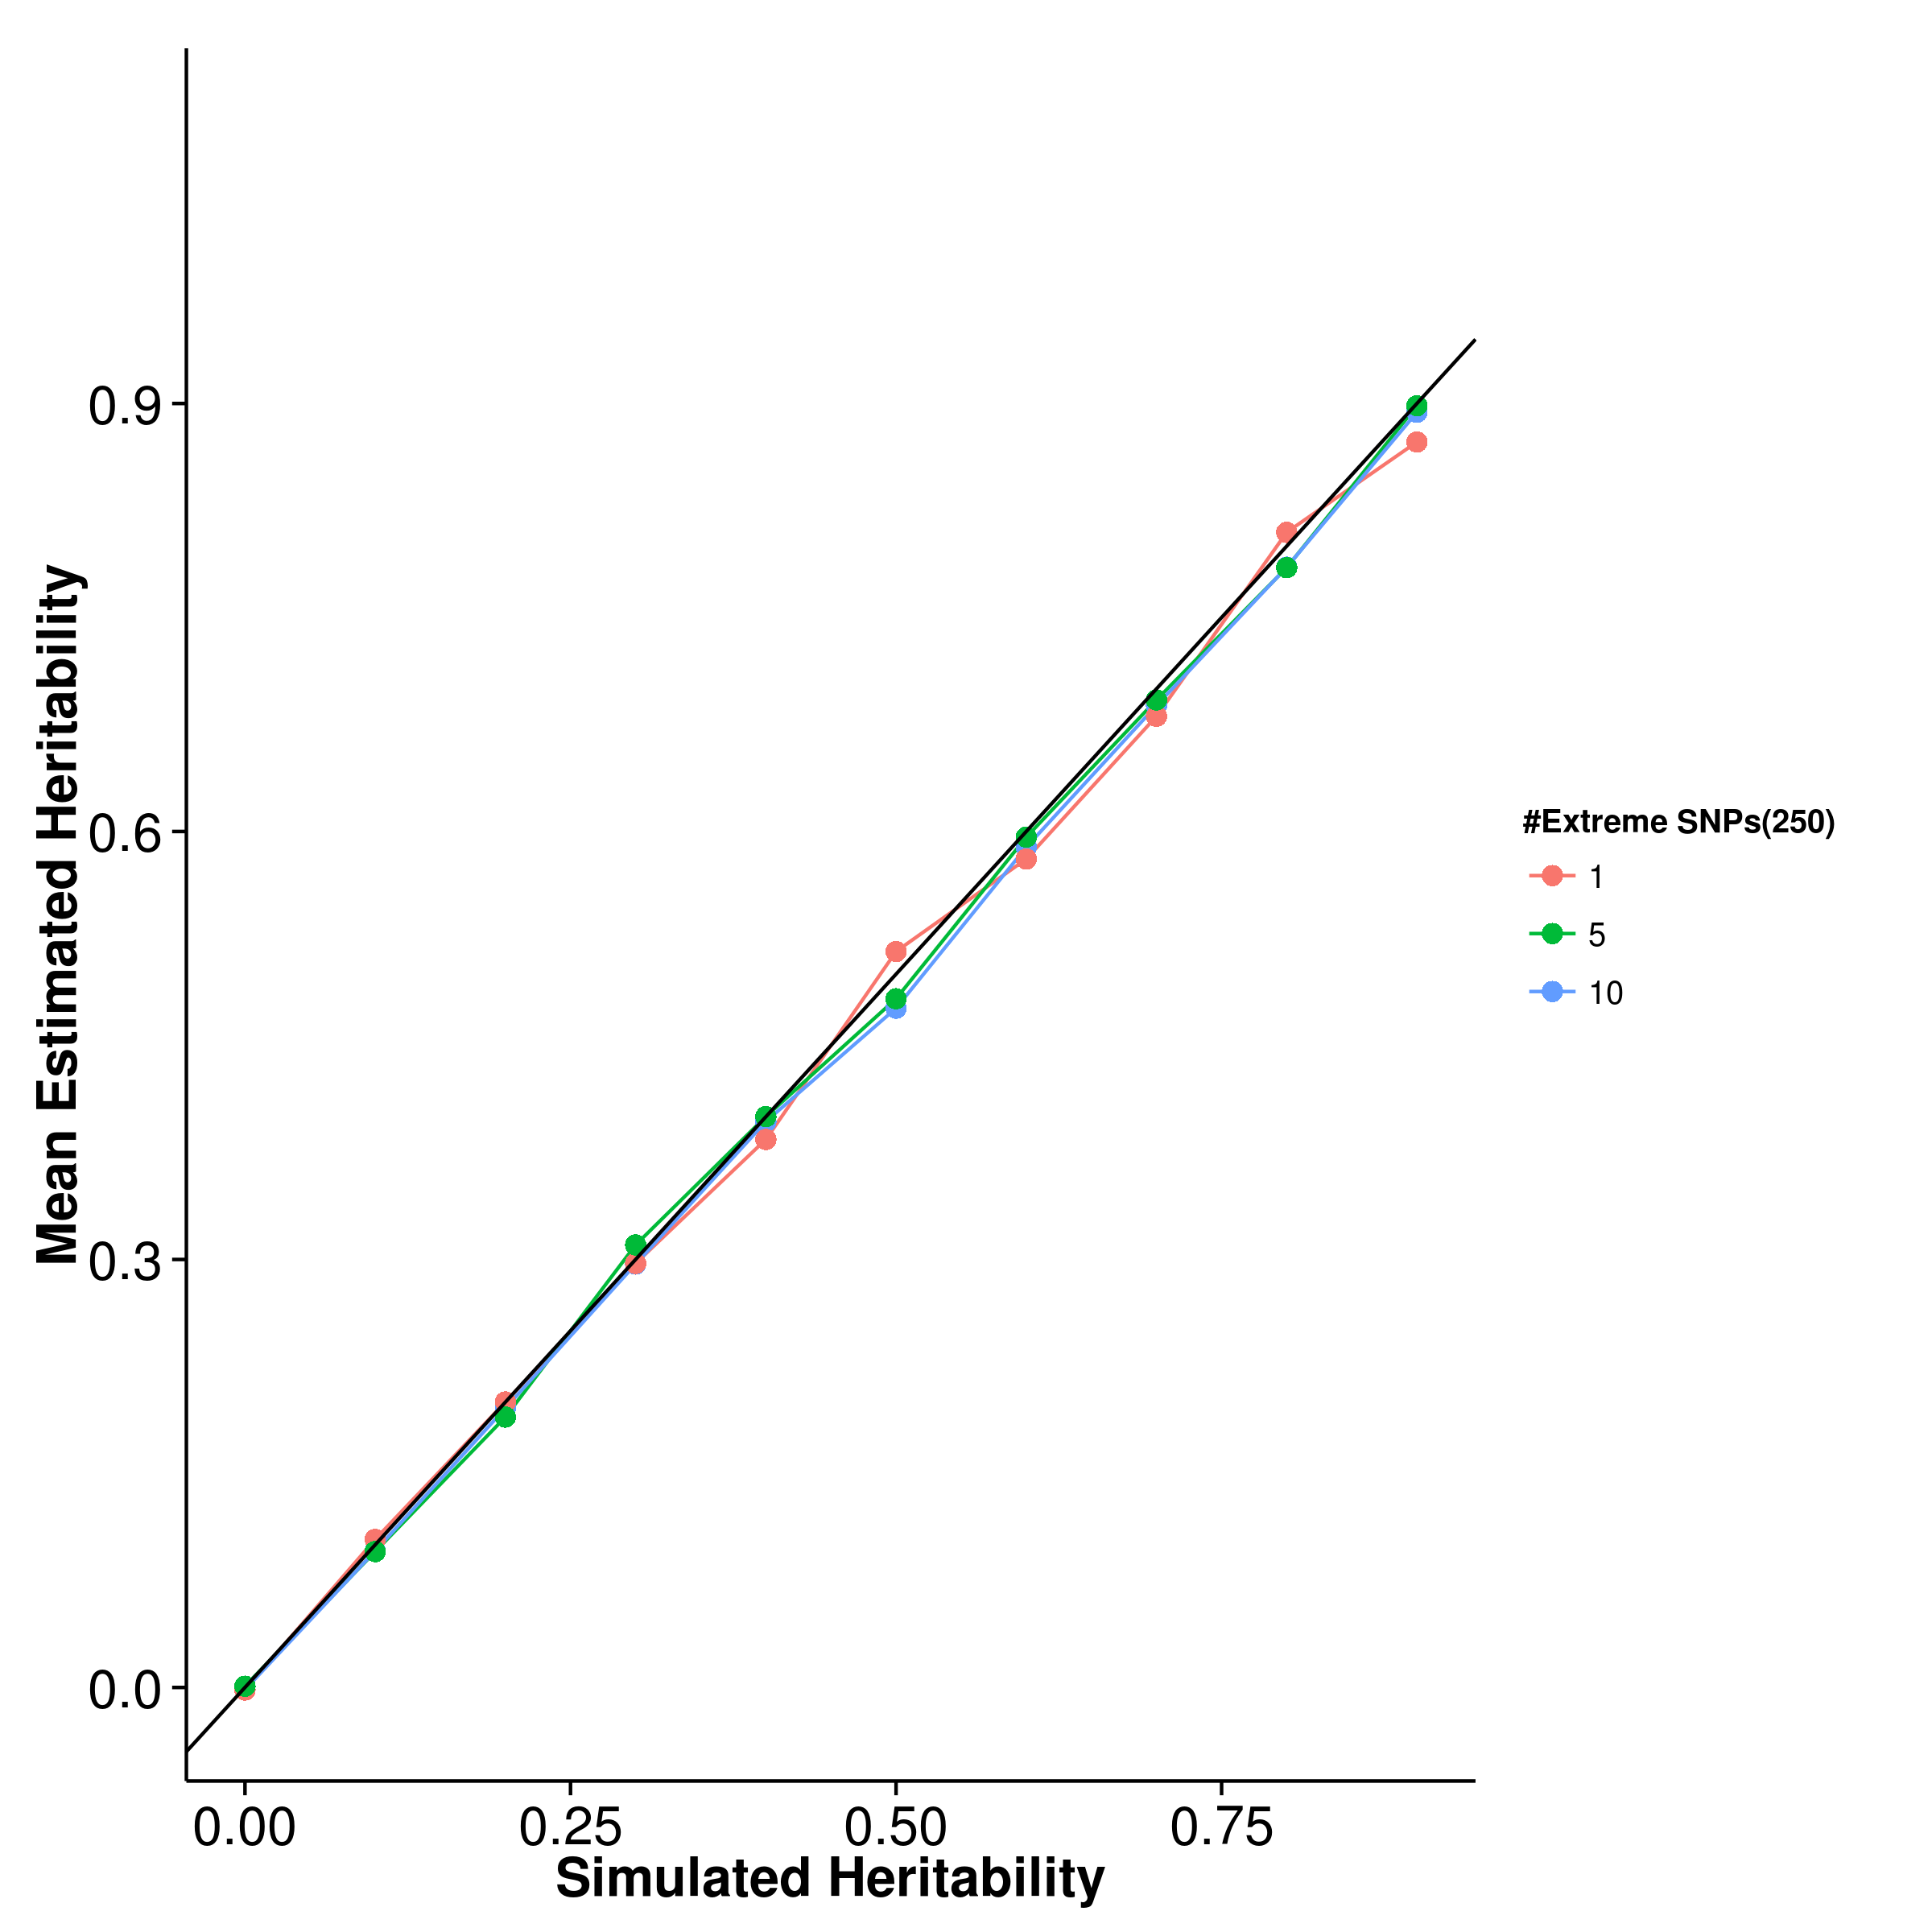
\includegraphics{figure/he_summary/extreme_250c/shrek_QtE_Extreme_mean.png}}
				\label{fig:shrekQtEx250cMean}
			}
			\subfloat[GCTA]{
				\scalebox{.4}{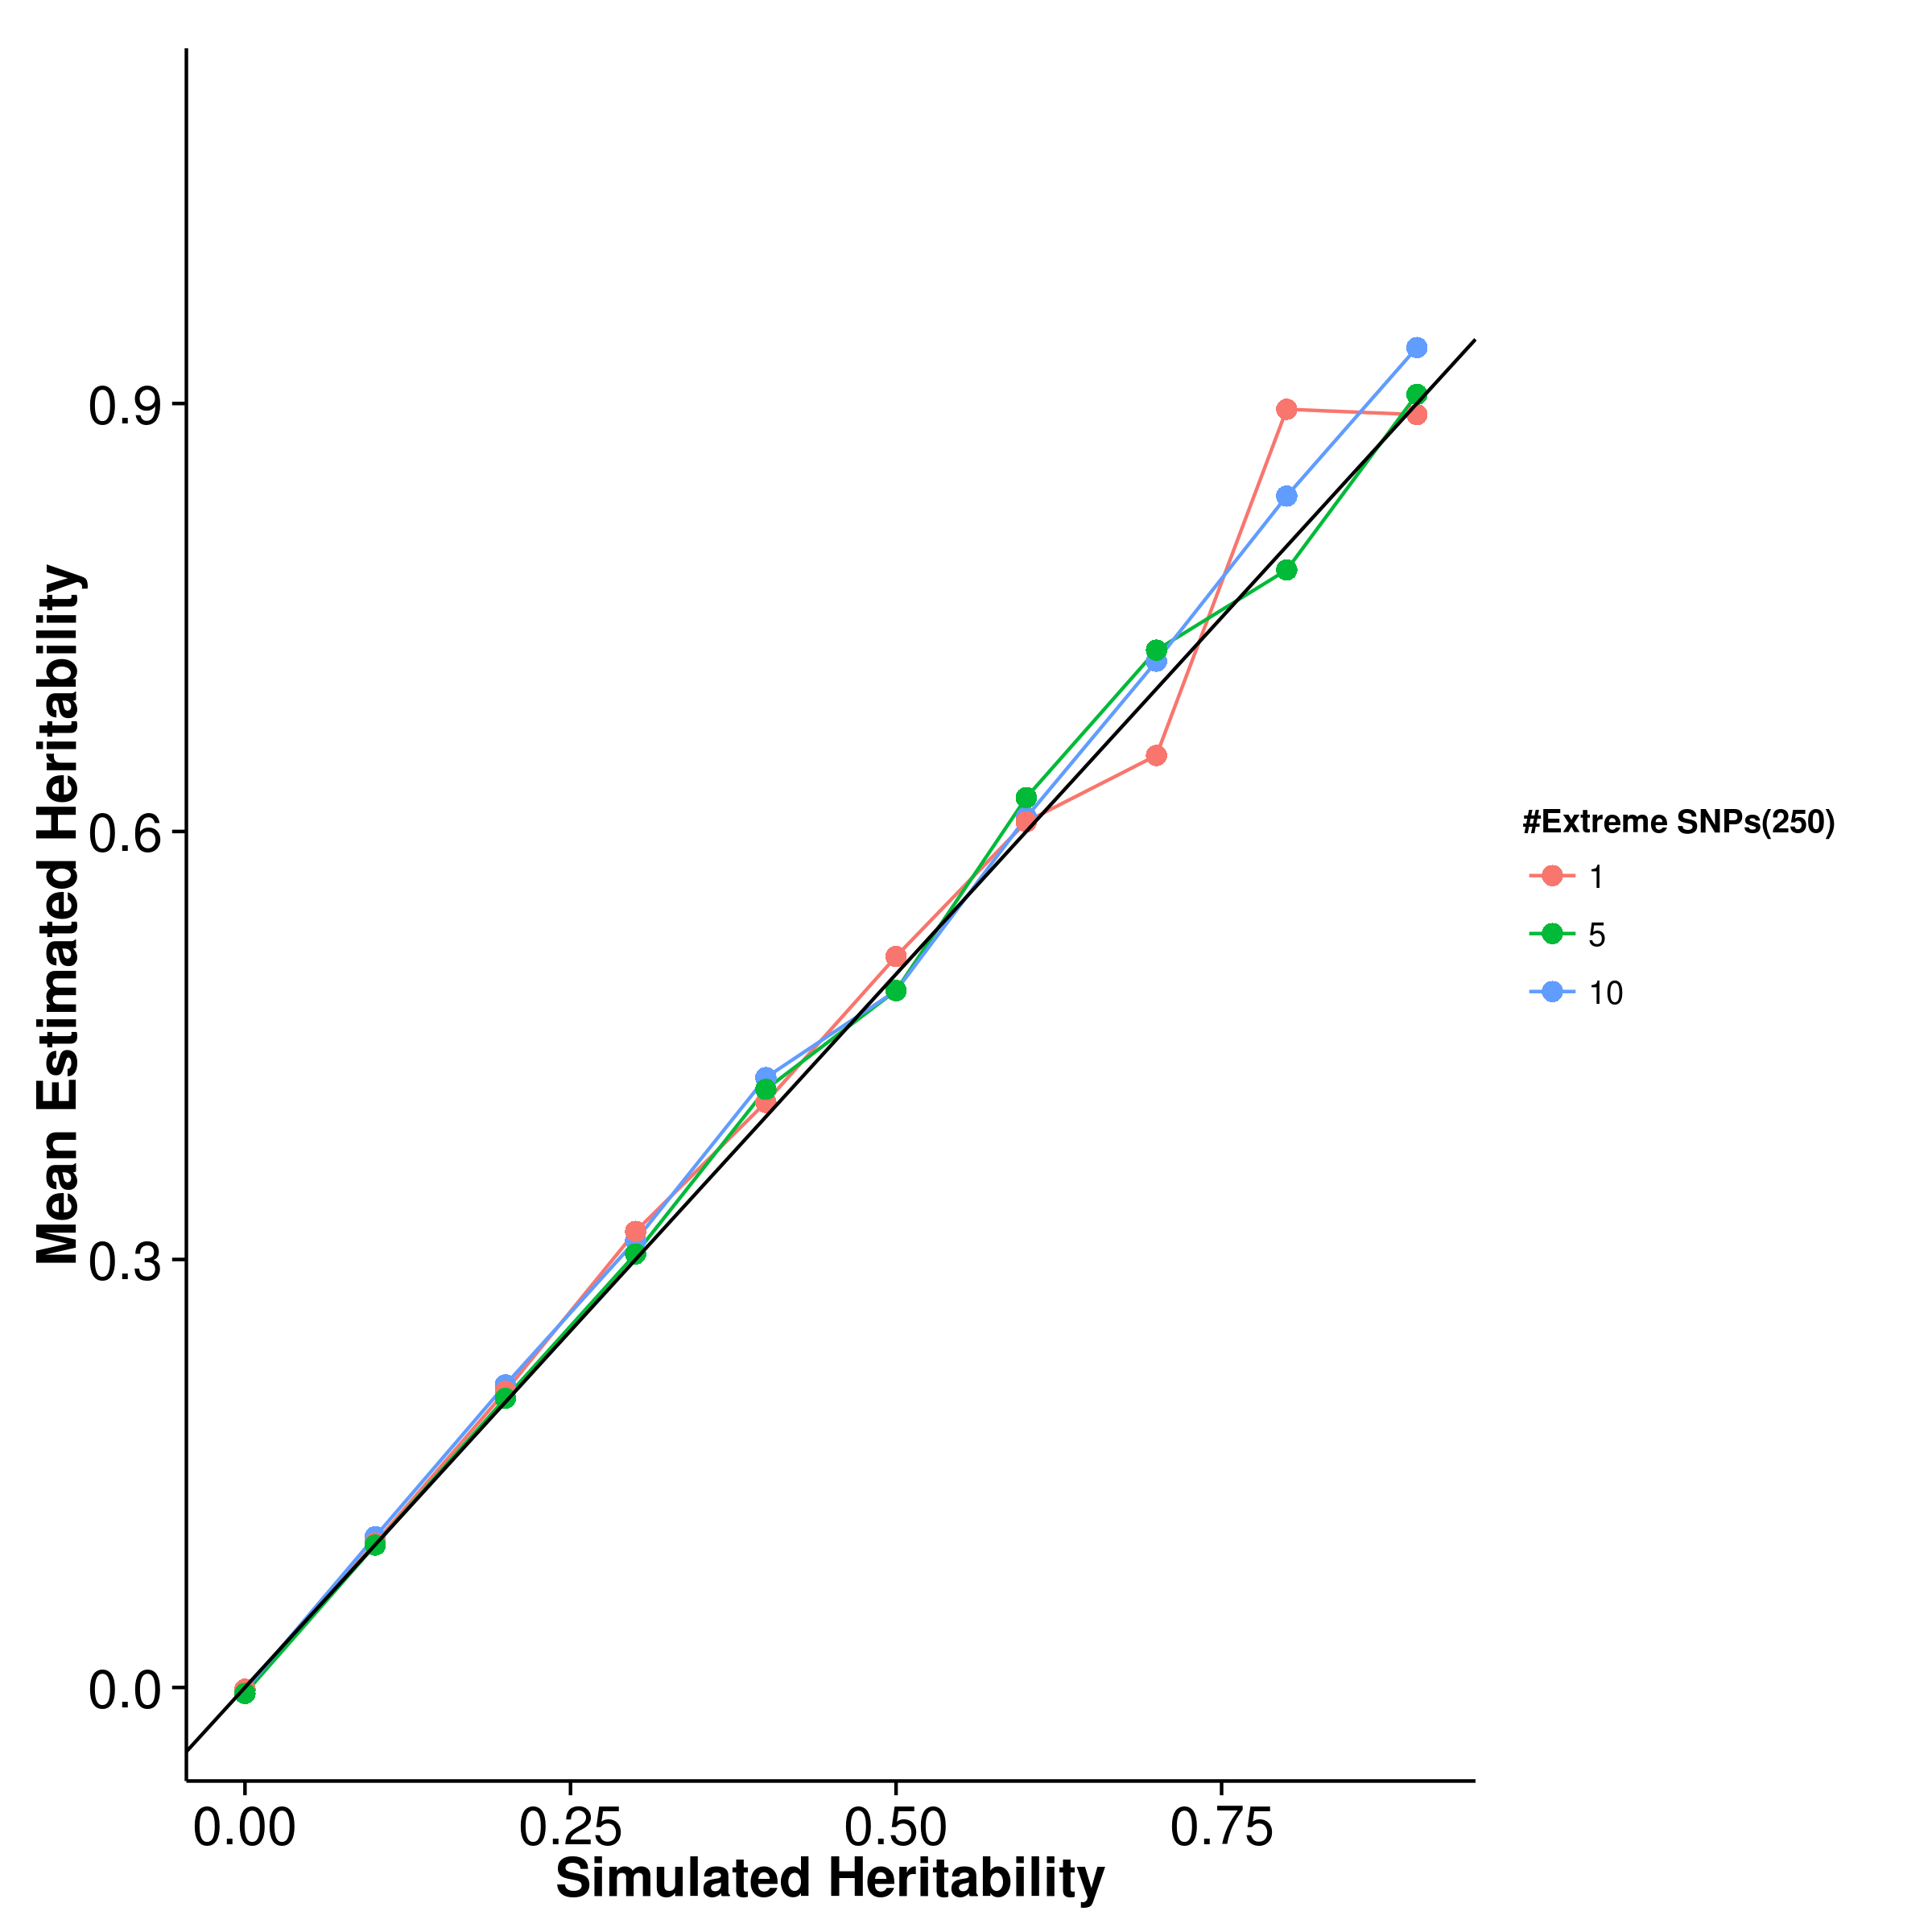
\includegraphics{figure/he_summary/extreme_250c/gcta_QtE_Extreme_mean.png}}
				\label{fig:gctaQtEx250cMean}
			}\\
			\subfloat[LDSC with fix intercept]{
				\scalebox{.4}{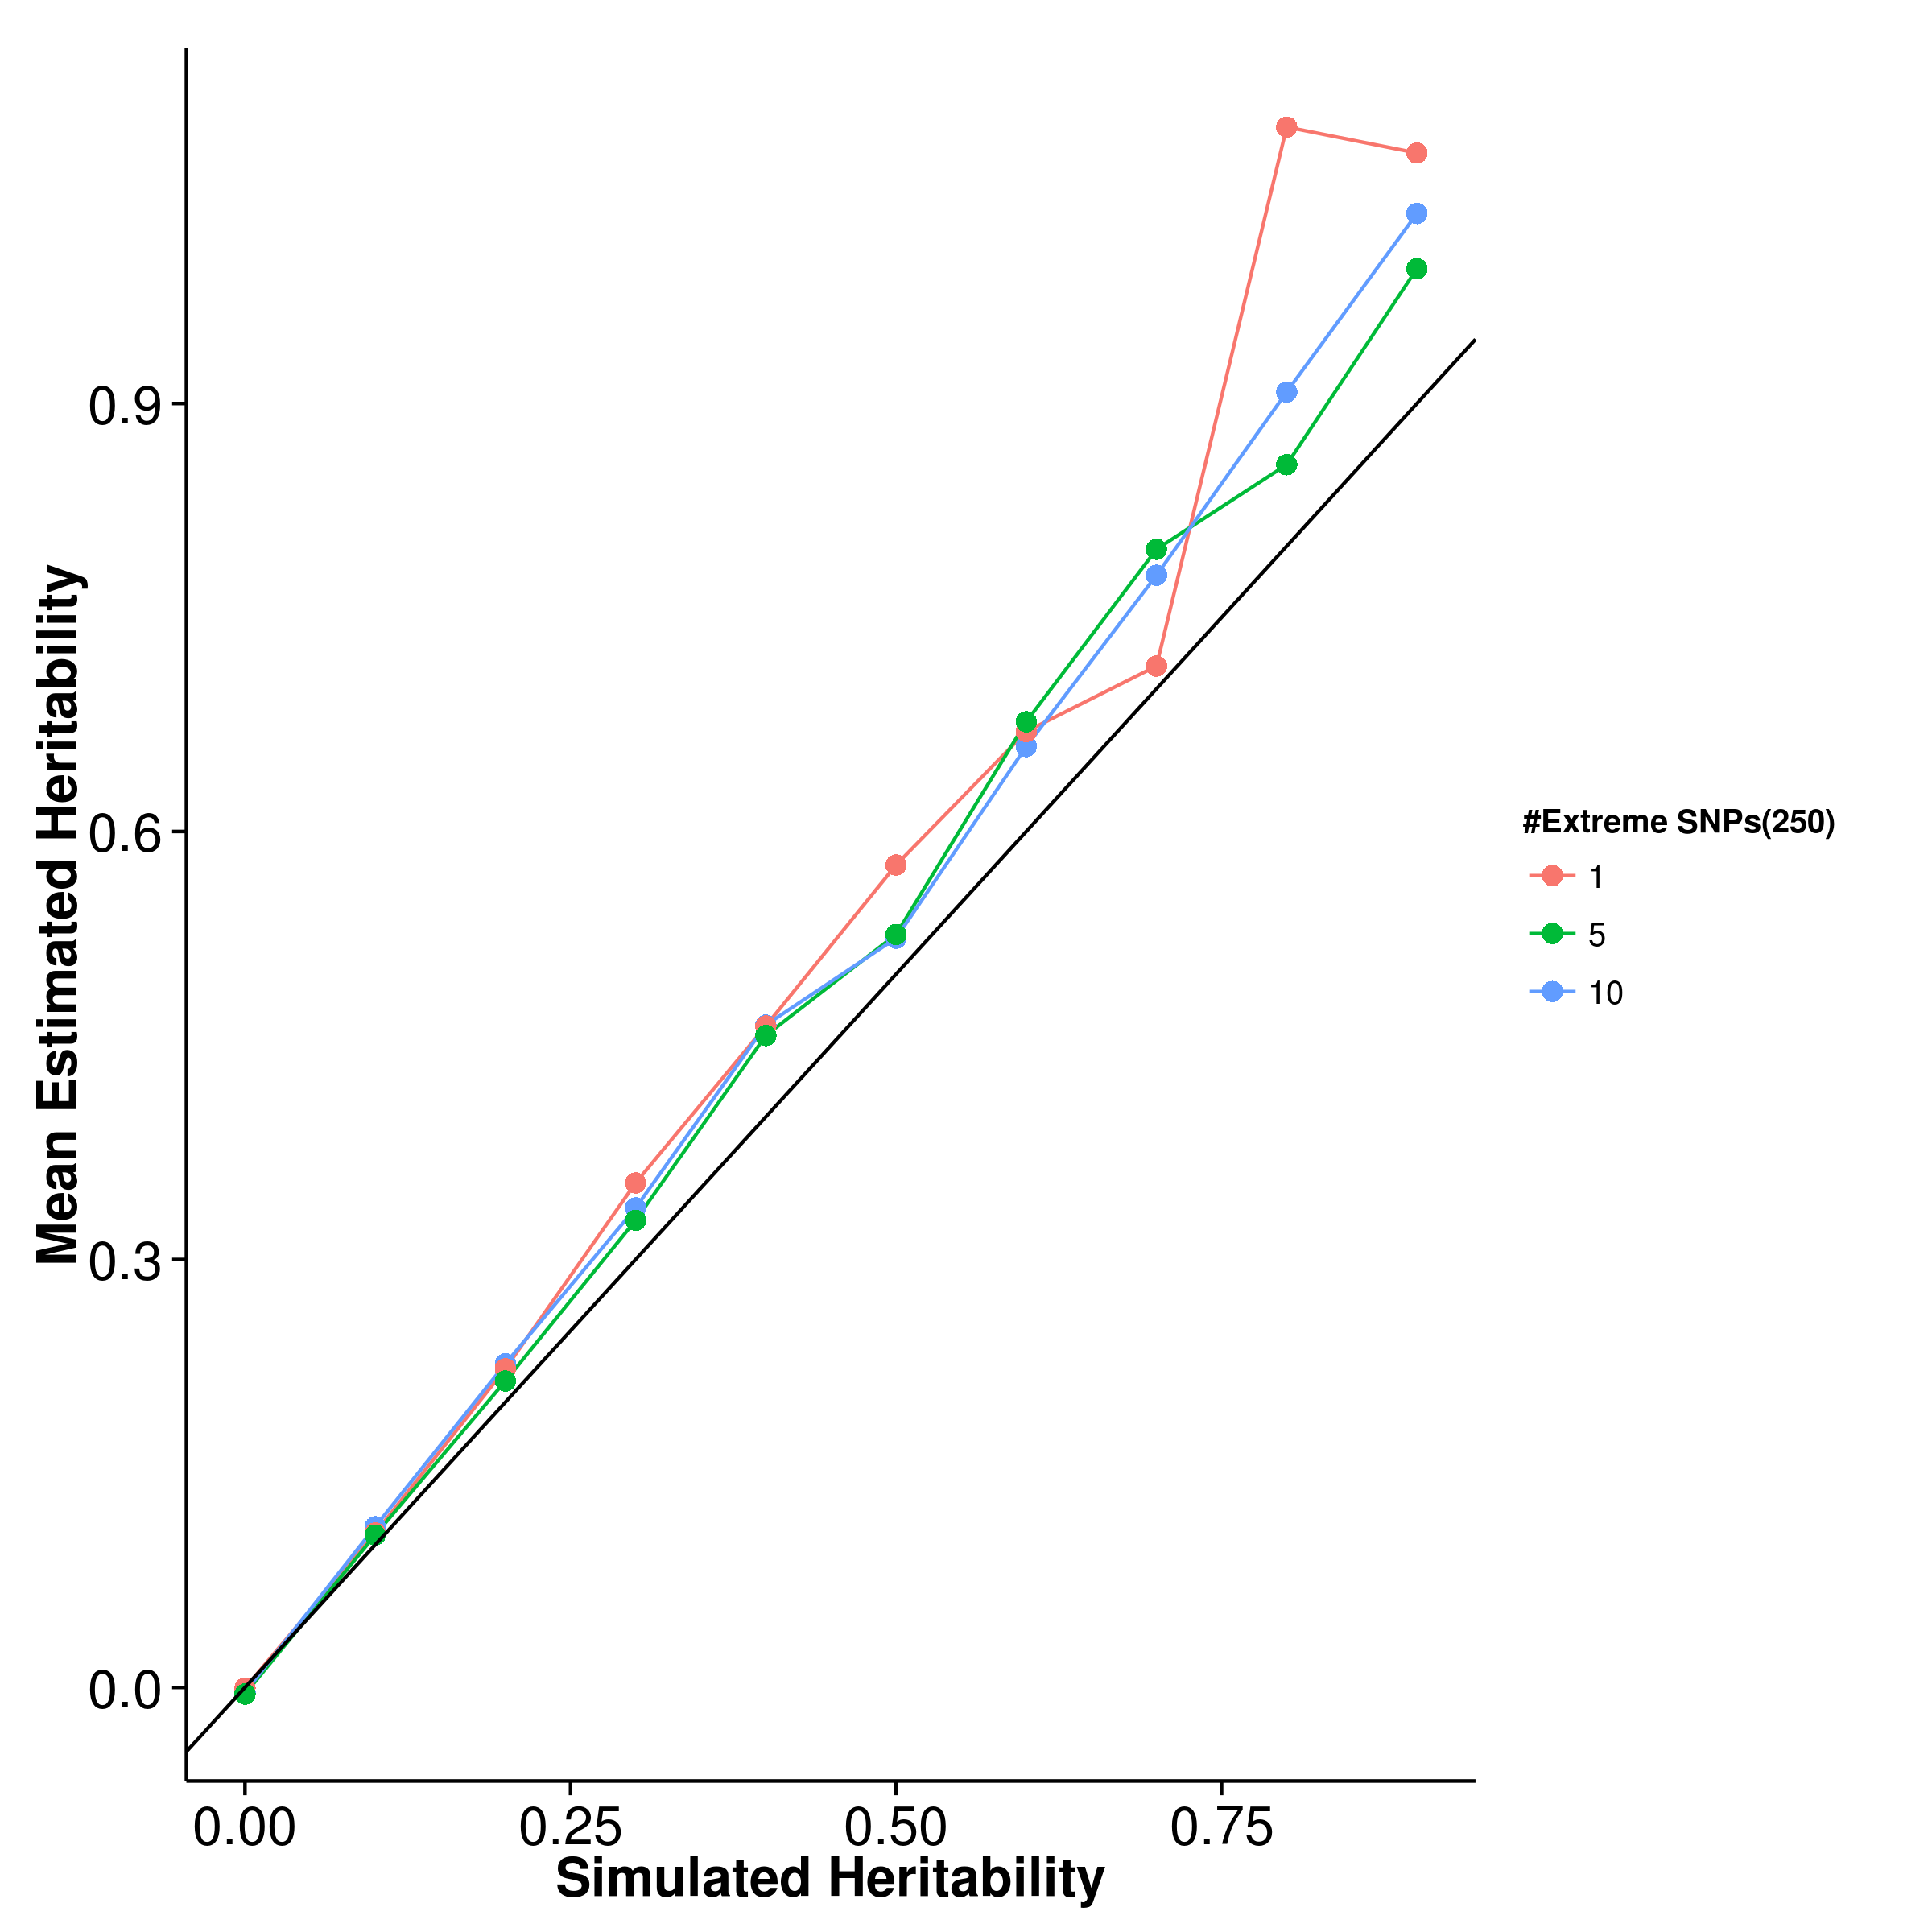
\includegraphics{figure/he_summary/extreme_250c/ldsc_QtE_Extreme_mean.png}}
				\label{fig:ldscQtEx250cMean}
			}
			\subfloat[LDSC with intercept estimation]{
				
				\scalebox{.4}{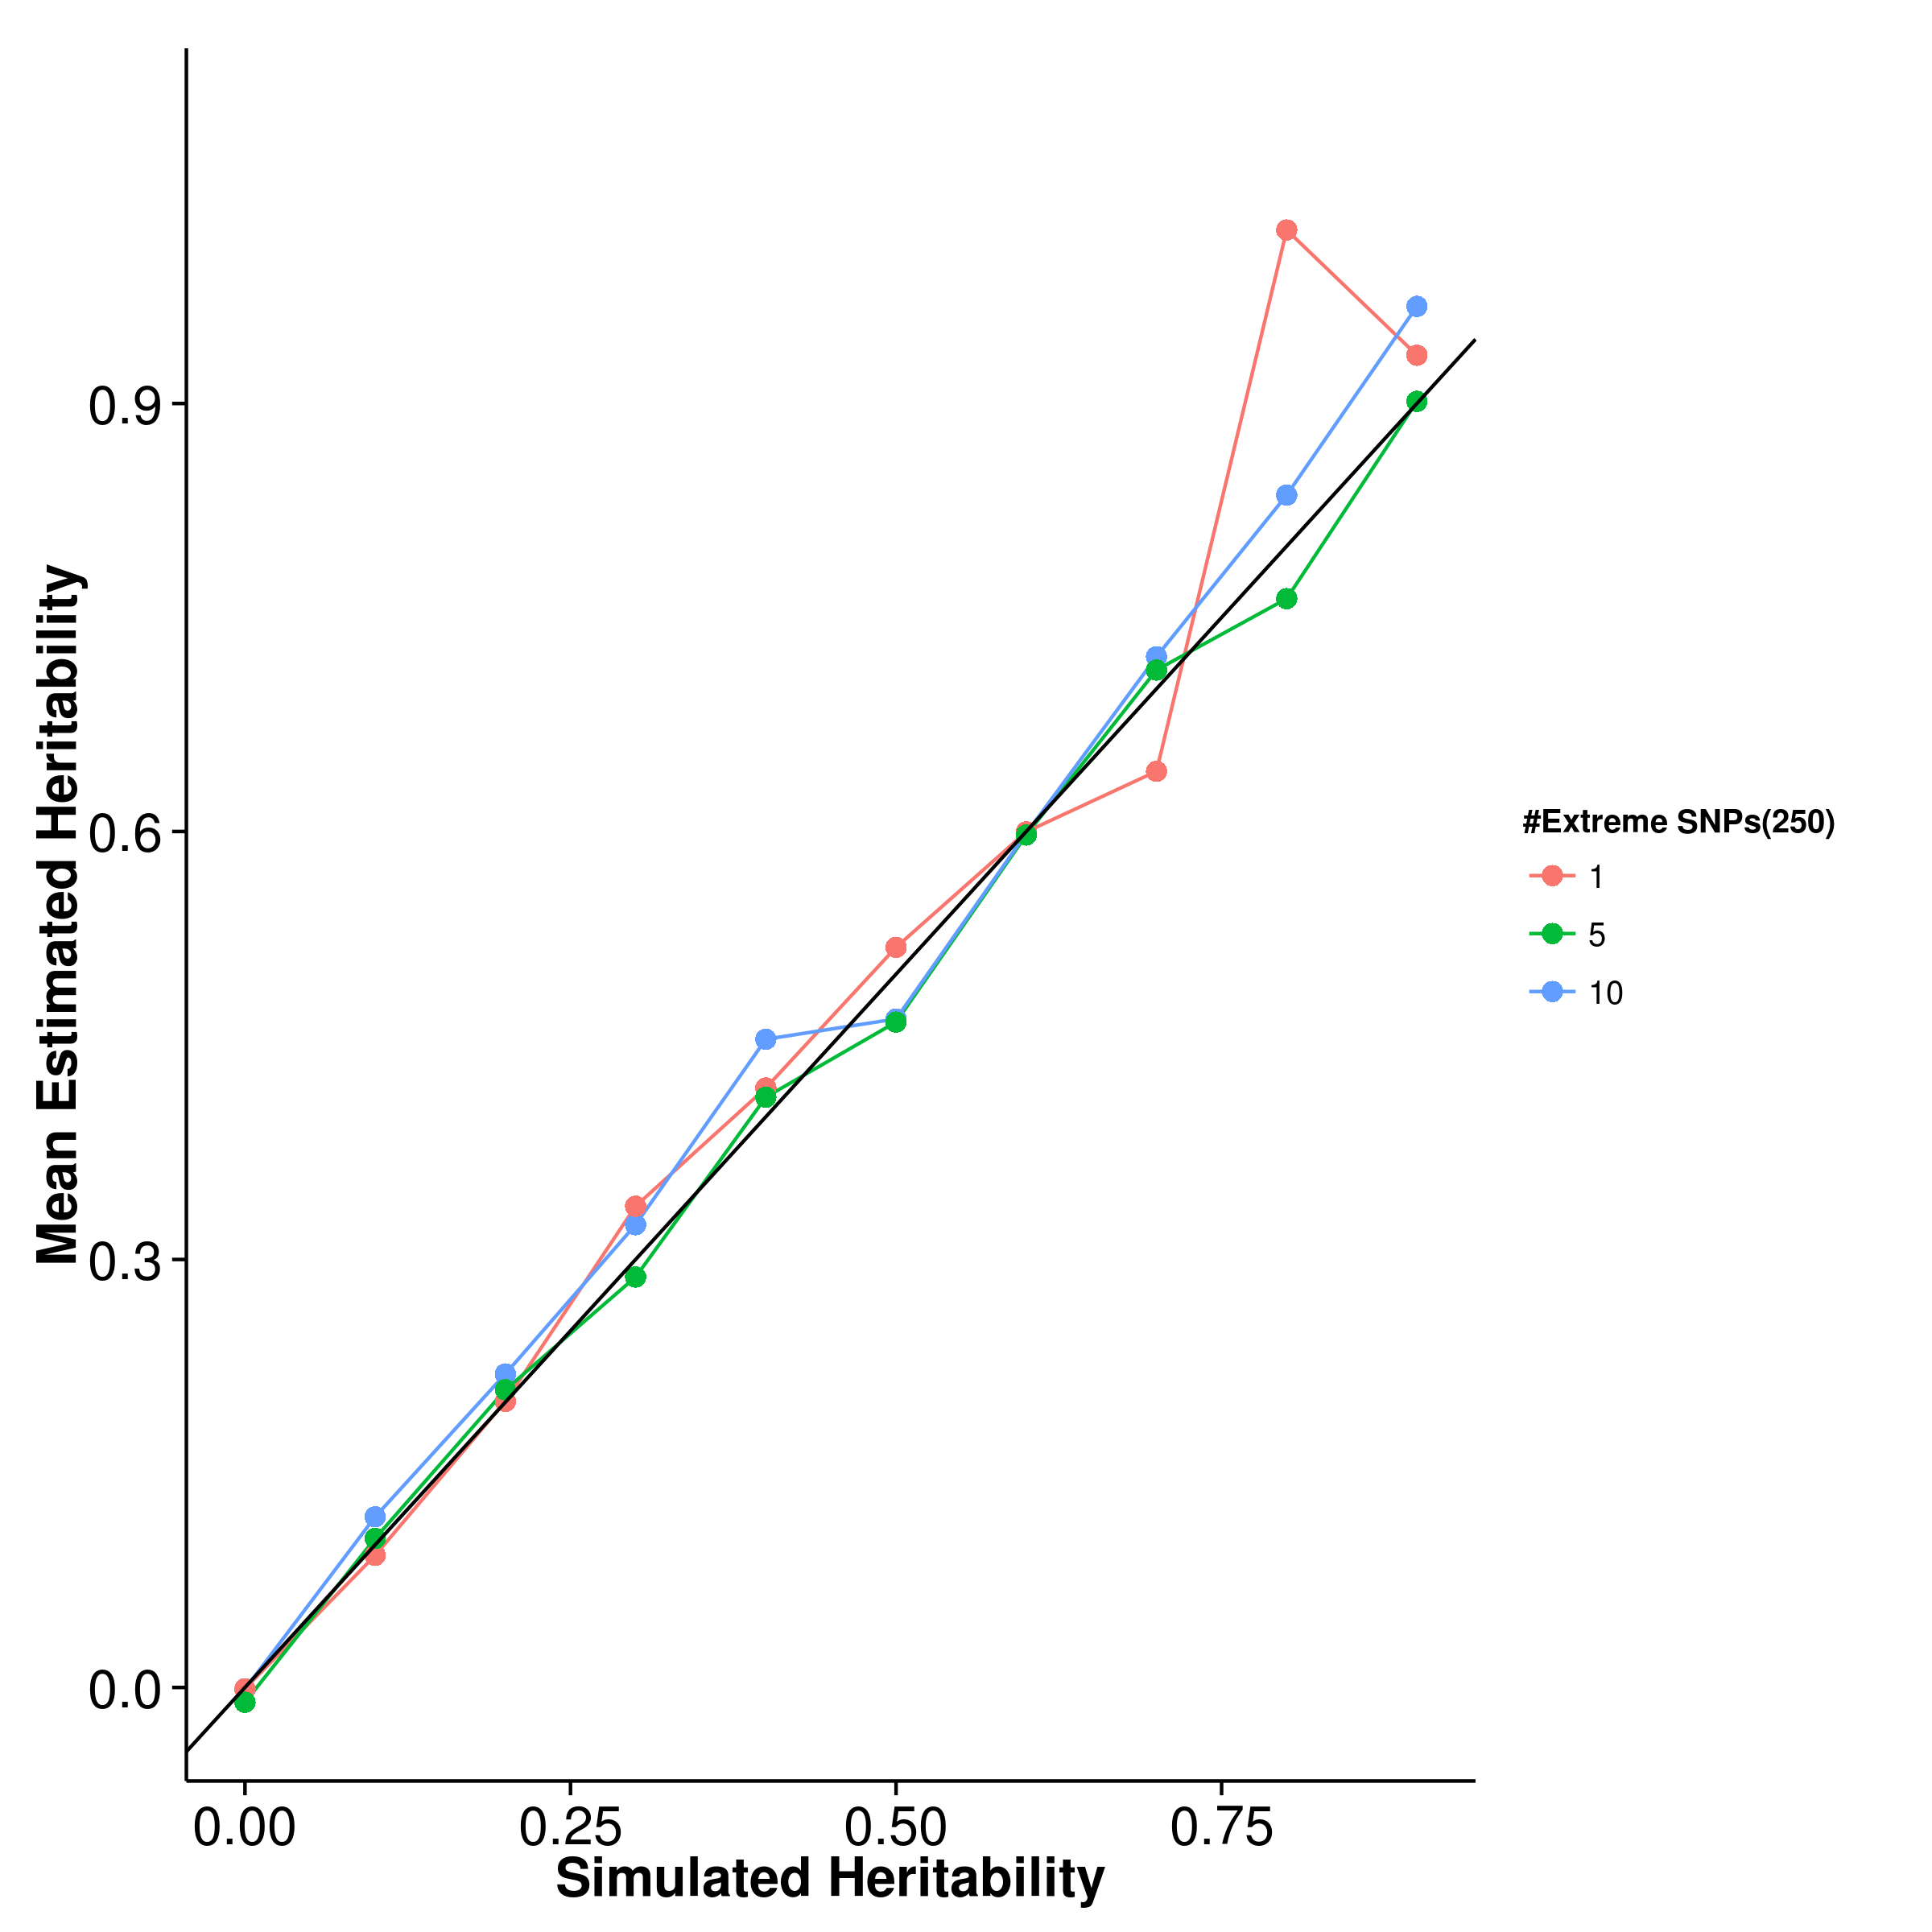
\includegraphics{figure/he_summary/extreme_250c/ldscIn_QtE_Extreme_mean.png}}
				\label{fig:ldscInQtEx250cMean}
			}
			\caption[Quantitative Trait with Extreme Effect Size Simulation Result(250 causal SNPs, Mean)]
			{Mean of results from quantitative trait simulation with extreme effect size simulation.
				250 causal \glspl{SNP} were simulated.
				It was observed that the mean estimation of heritability of all the tools were relatively unaffected by the number of \glspl{SNP} representing a large portion of effect, similar to what observed when 100 causal \glspl{SNP} were simulated.
				However, there seems to be an upward bias when \gls{ldsc} was performed with fixed intercept.
			} 
			\label{fig:QtEx250cMean}
		\end{figure}
		
		\begin{figure}
			\centering
			\subfloat[SHREK]{
				\scalebox{.4}{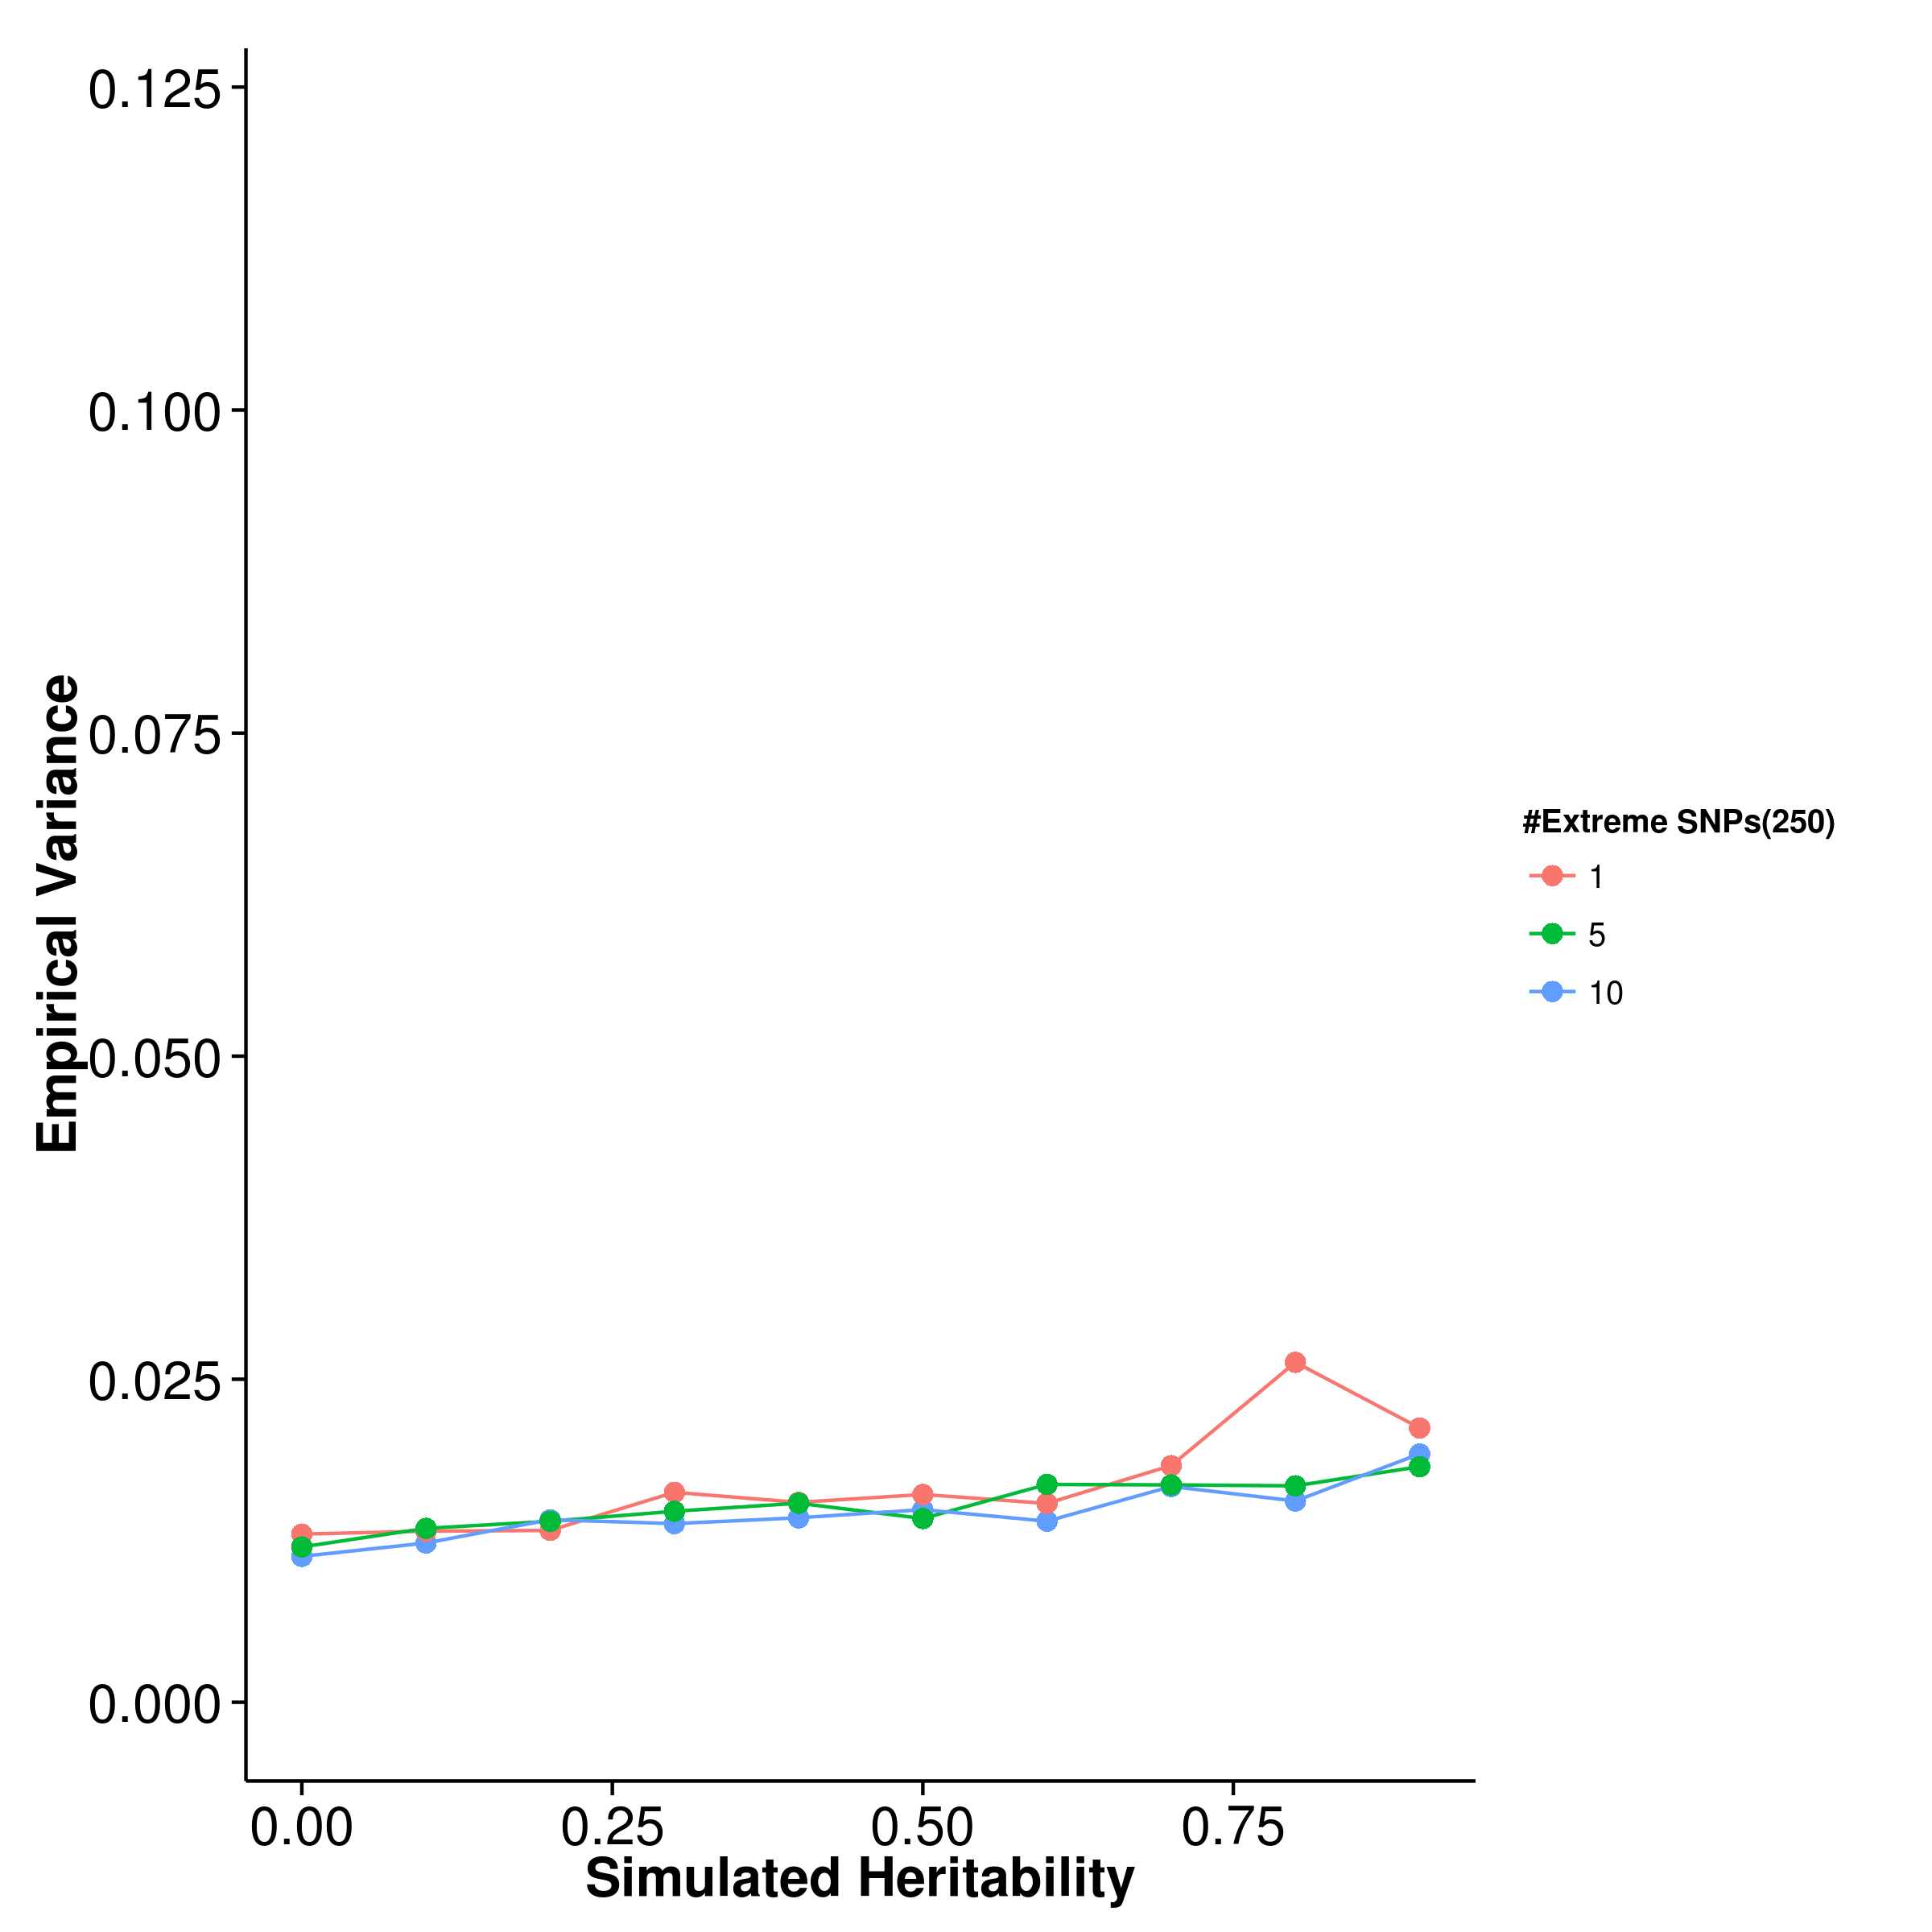
\includegraphics{figure/he_summary/extreme_250c/shrek_QtE_Extreme_sd.png}}
				\label{fig:shrekQtEx250cVar}
			}
			\subfloat[GCTA]{
				\scalebox{.4}{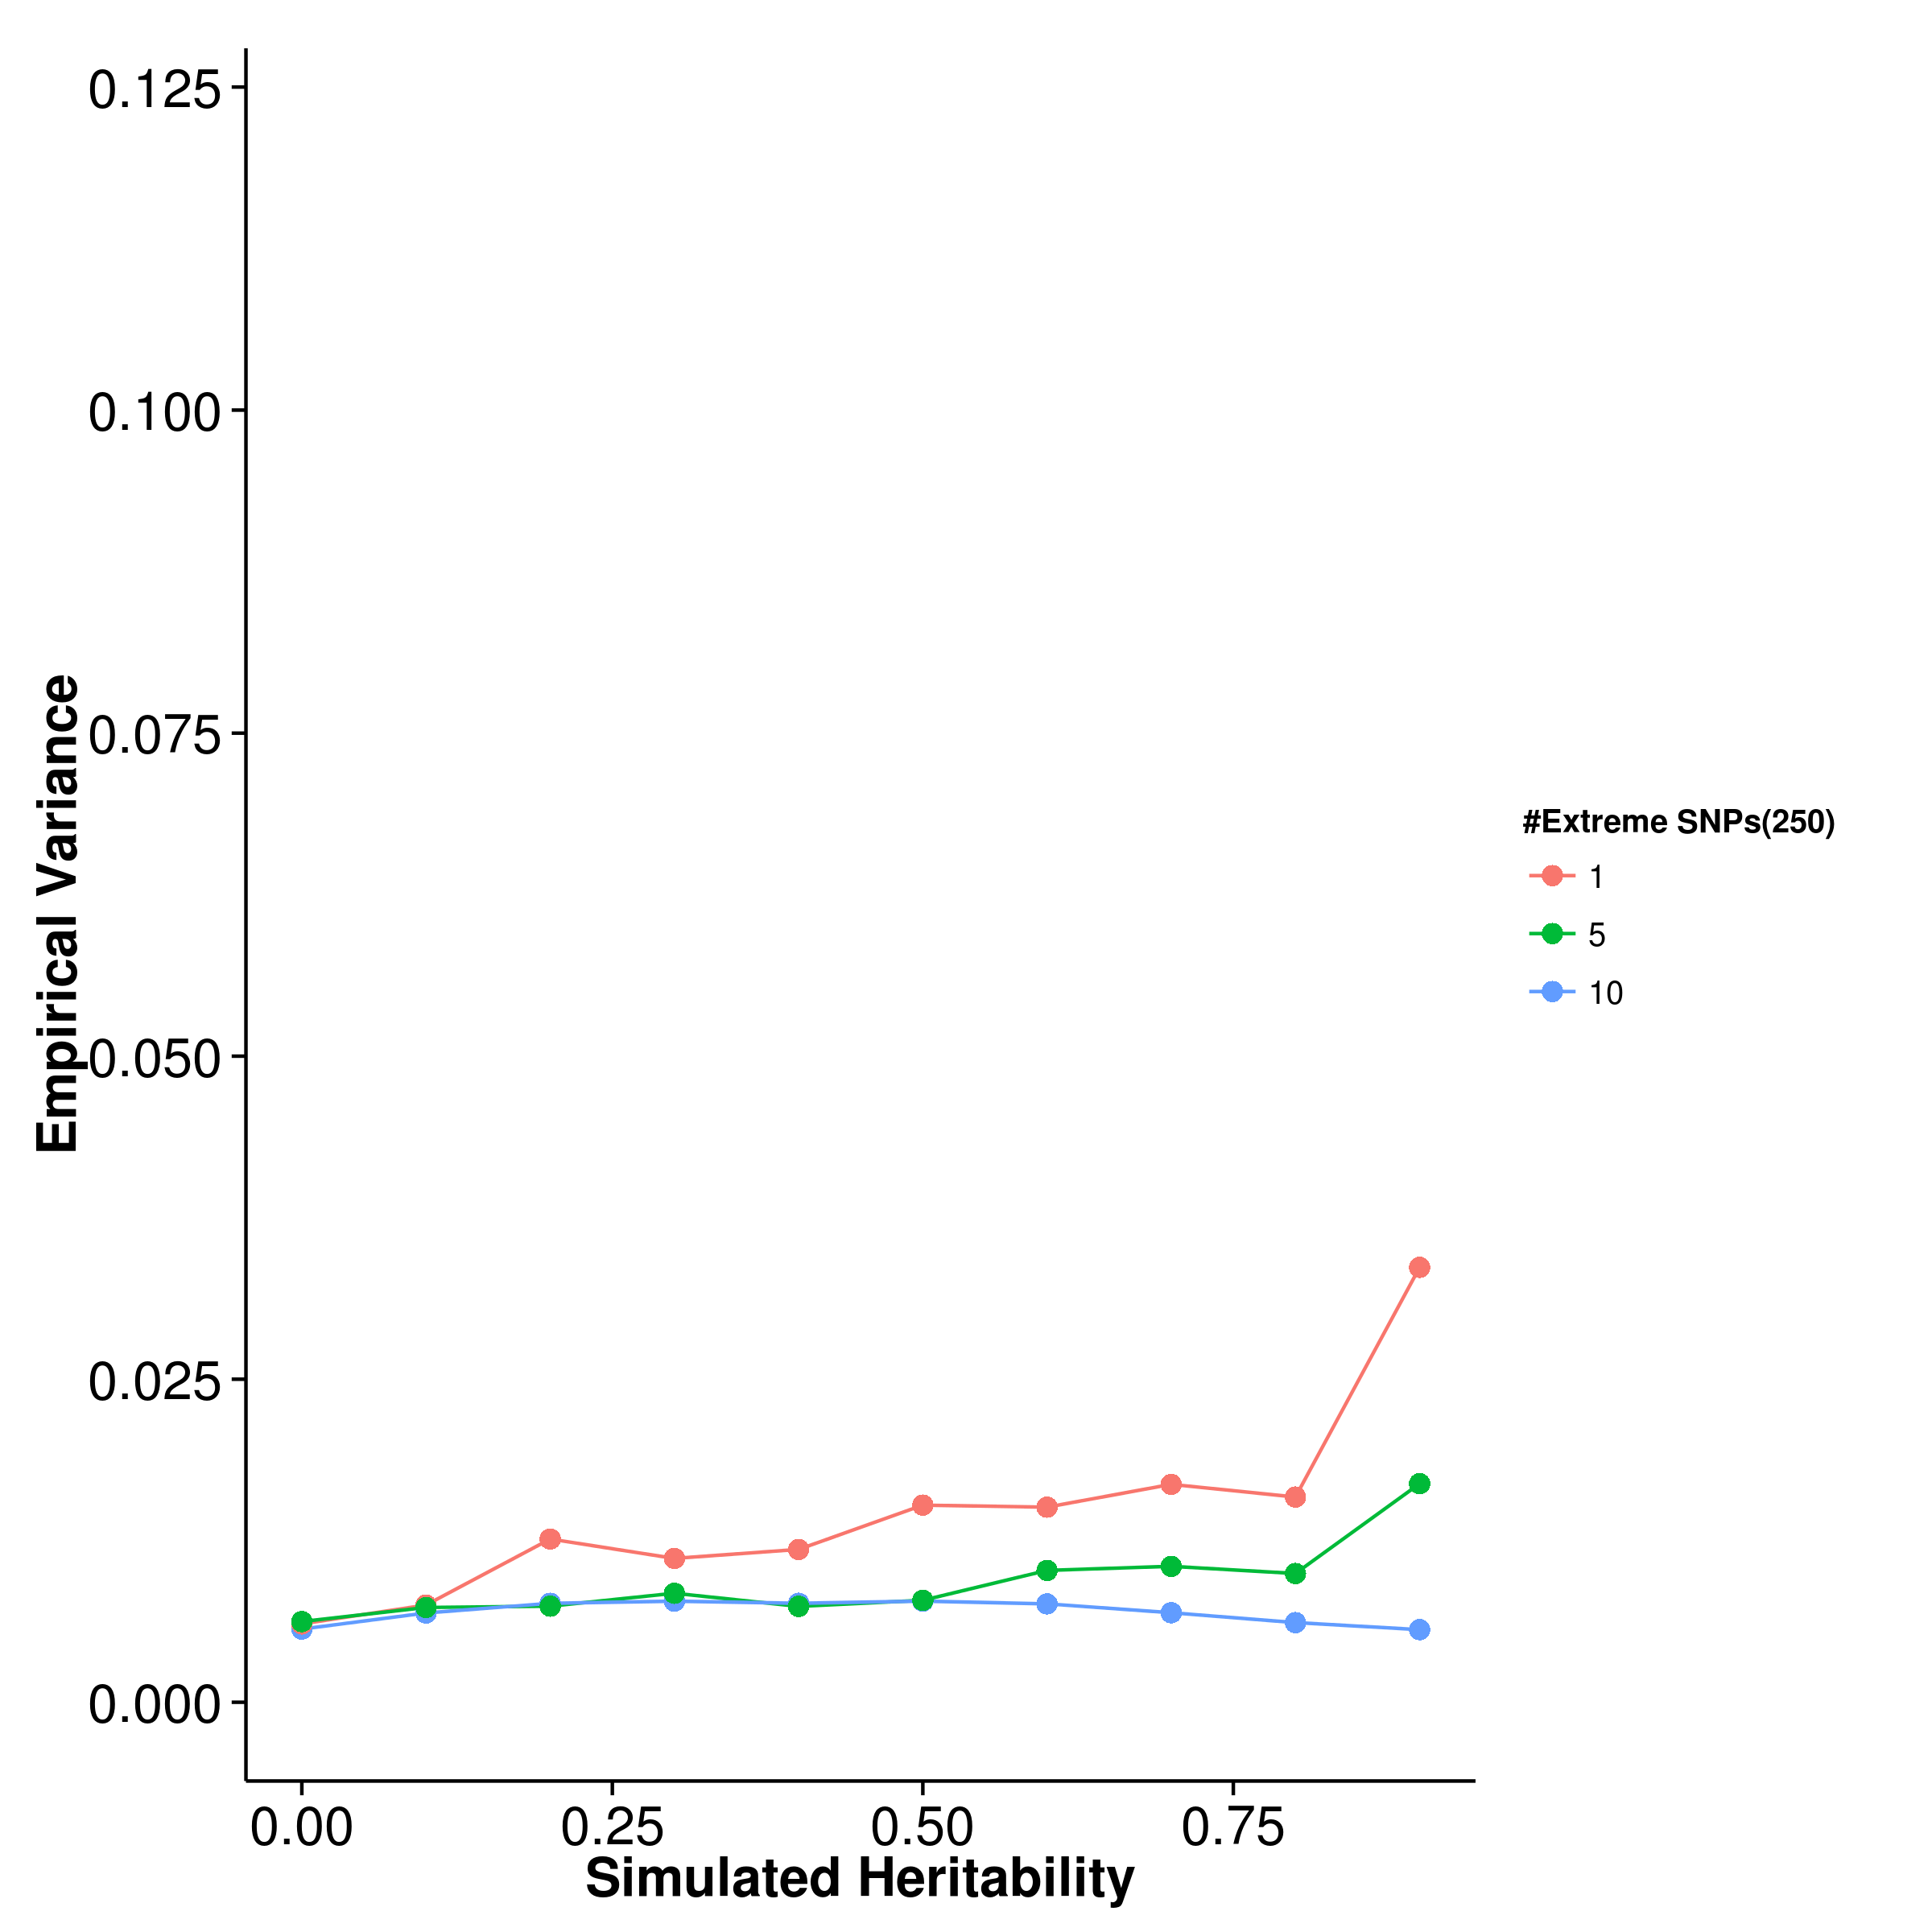
\includegraphics{figure/he_summary/extreme_250c/gcta_QtE_Extreme_sd.png}}
				\label{fig:gctaQtEx250cVar}
			}\\
			\subfloat[LDSC with fix intercept]{
				\scalebox{.4}{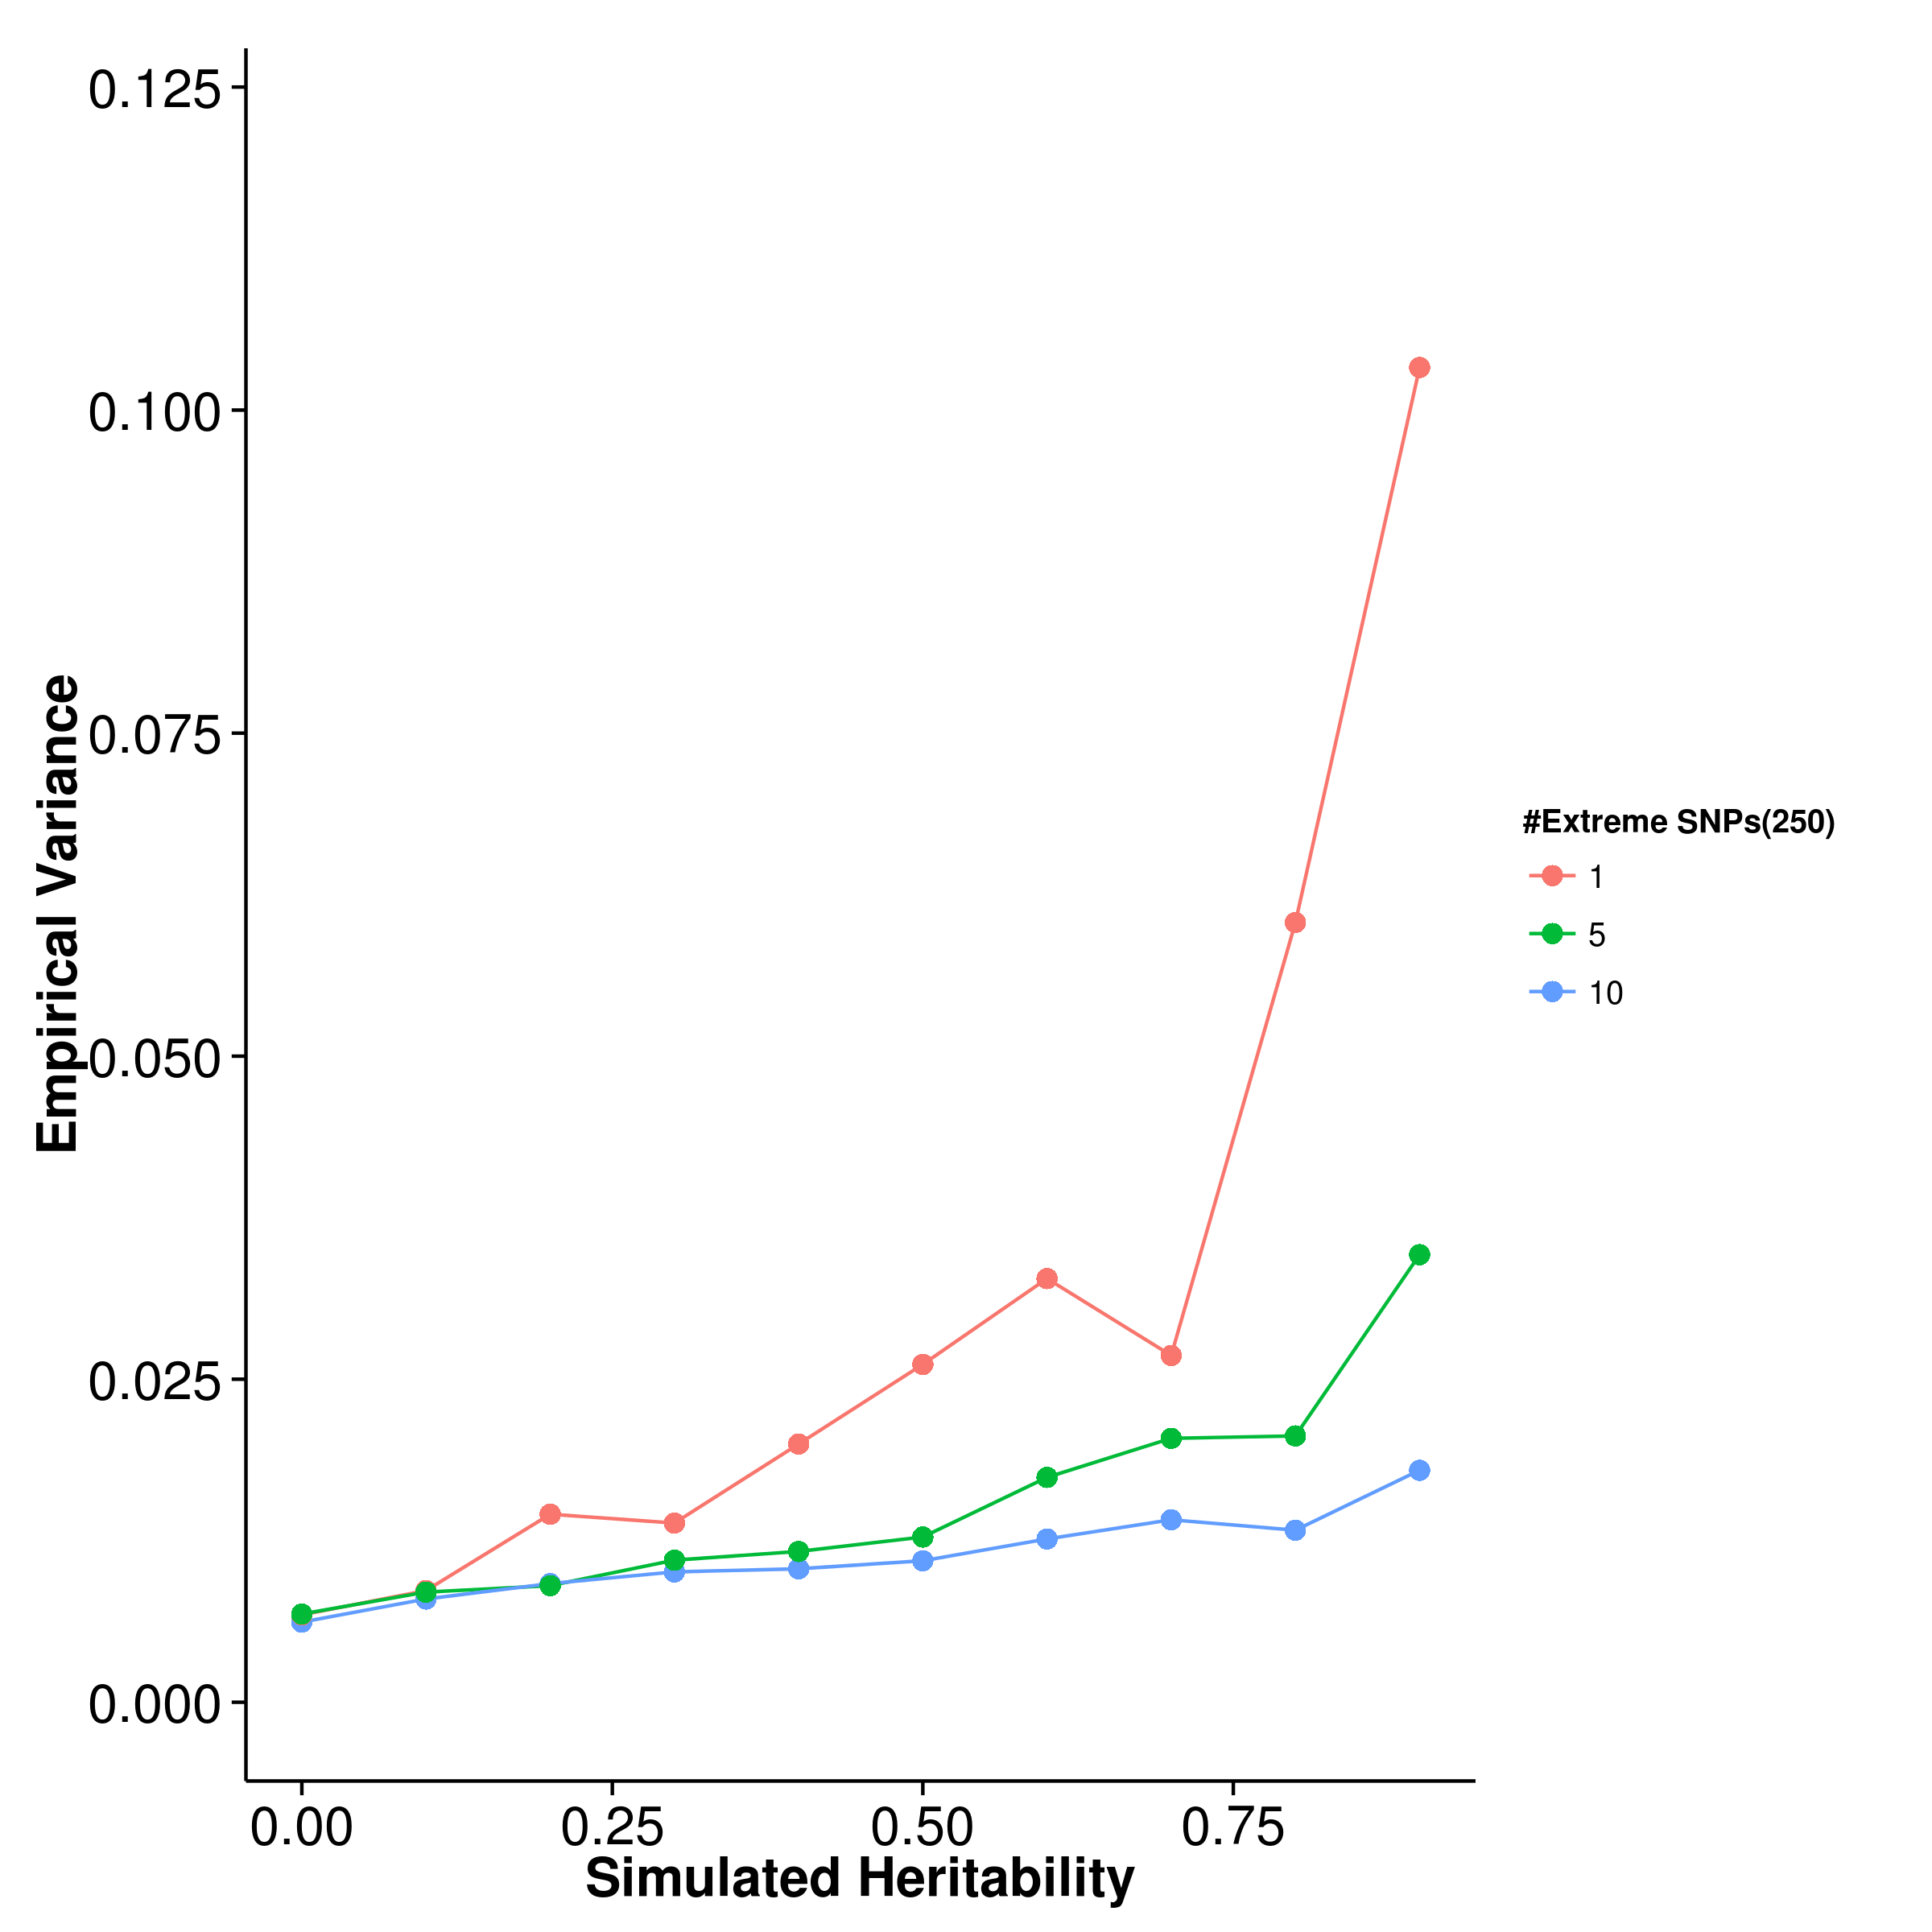
\includegraphics{figure/he_summary/extreme_250c/ldsc_QtE_Extreme_sd.png}}
				\label{fig:ldscQtEx250cVar}
			}
			\subfloat[LDSC with intercept estimation]{
				
				\scalebox{.4}{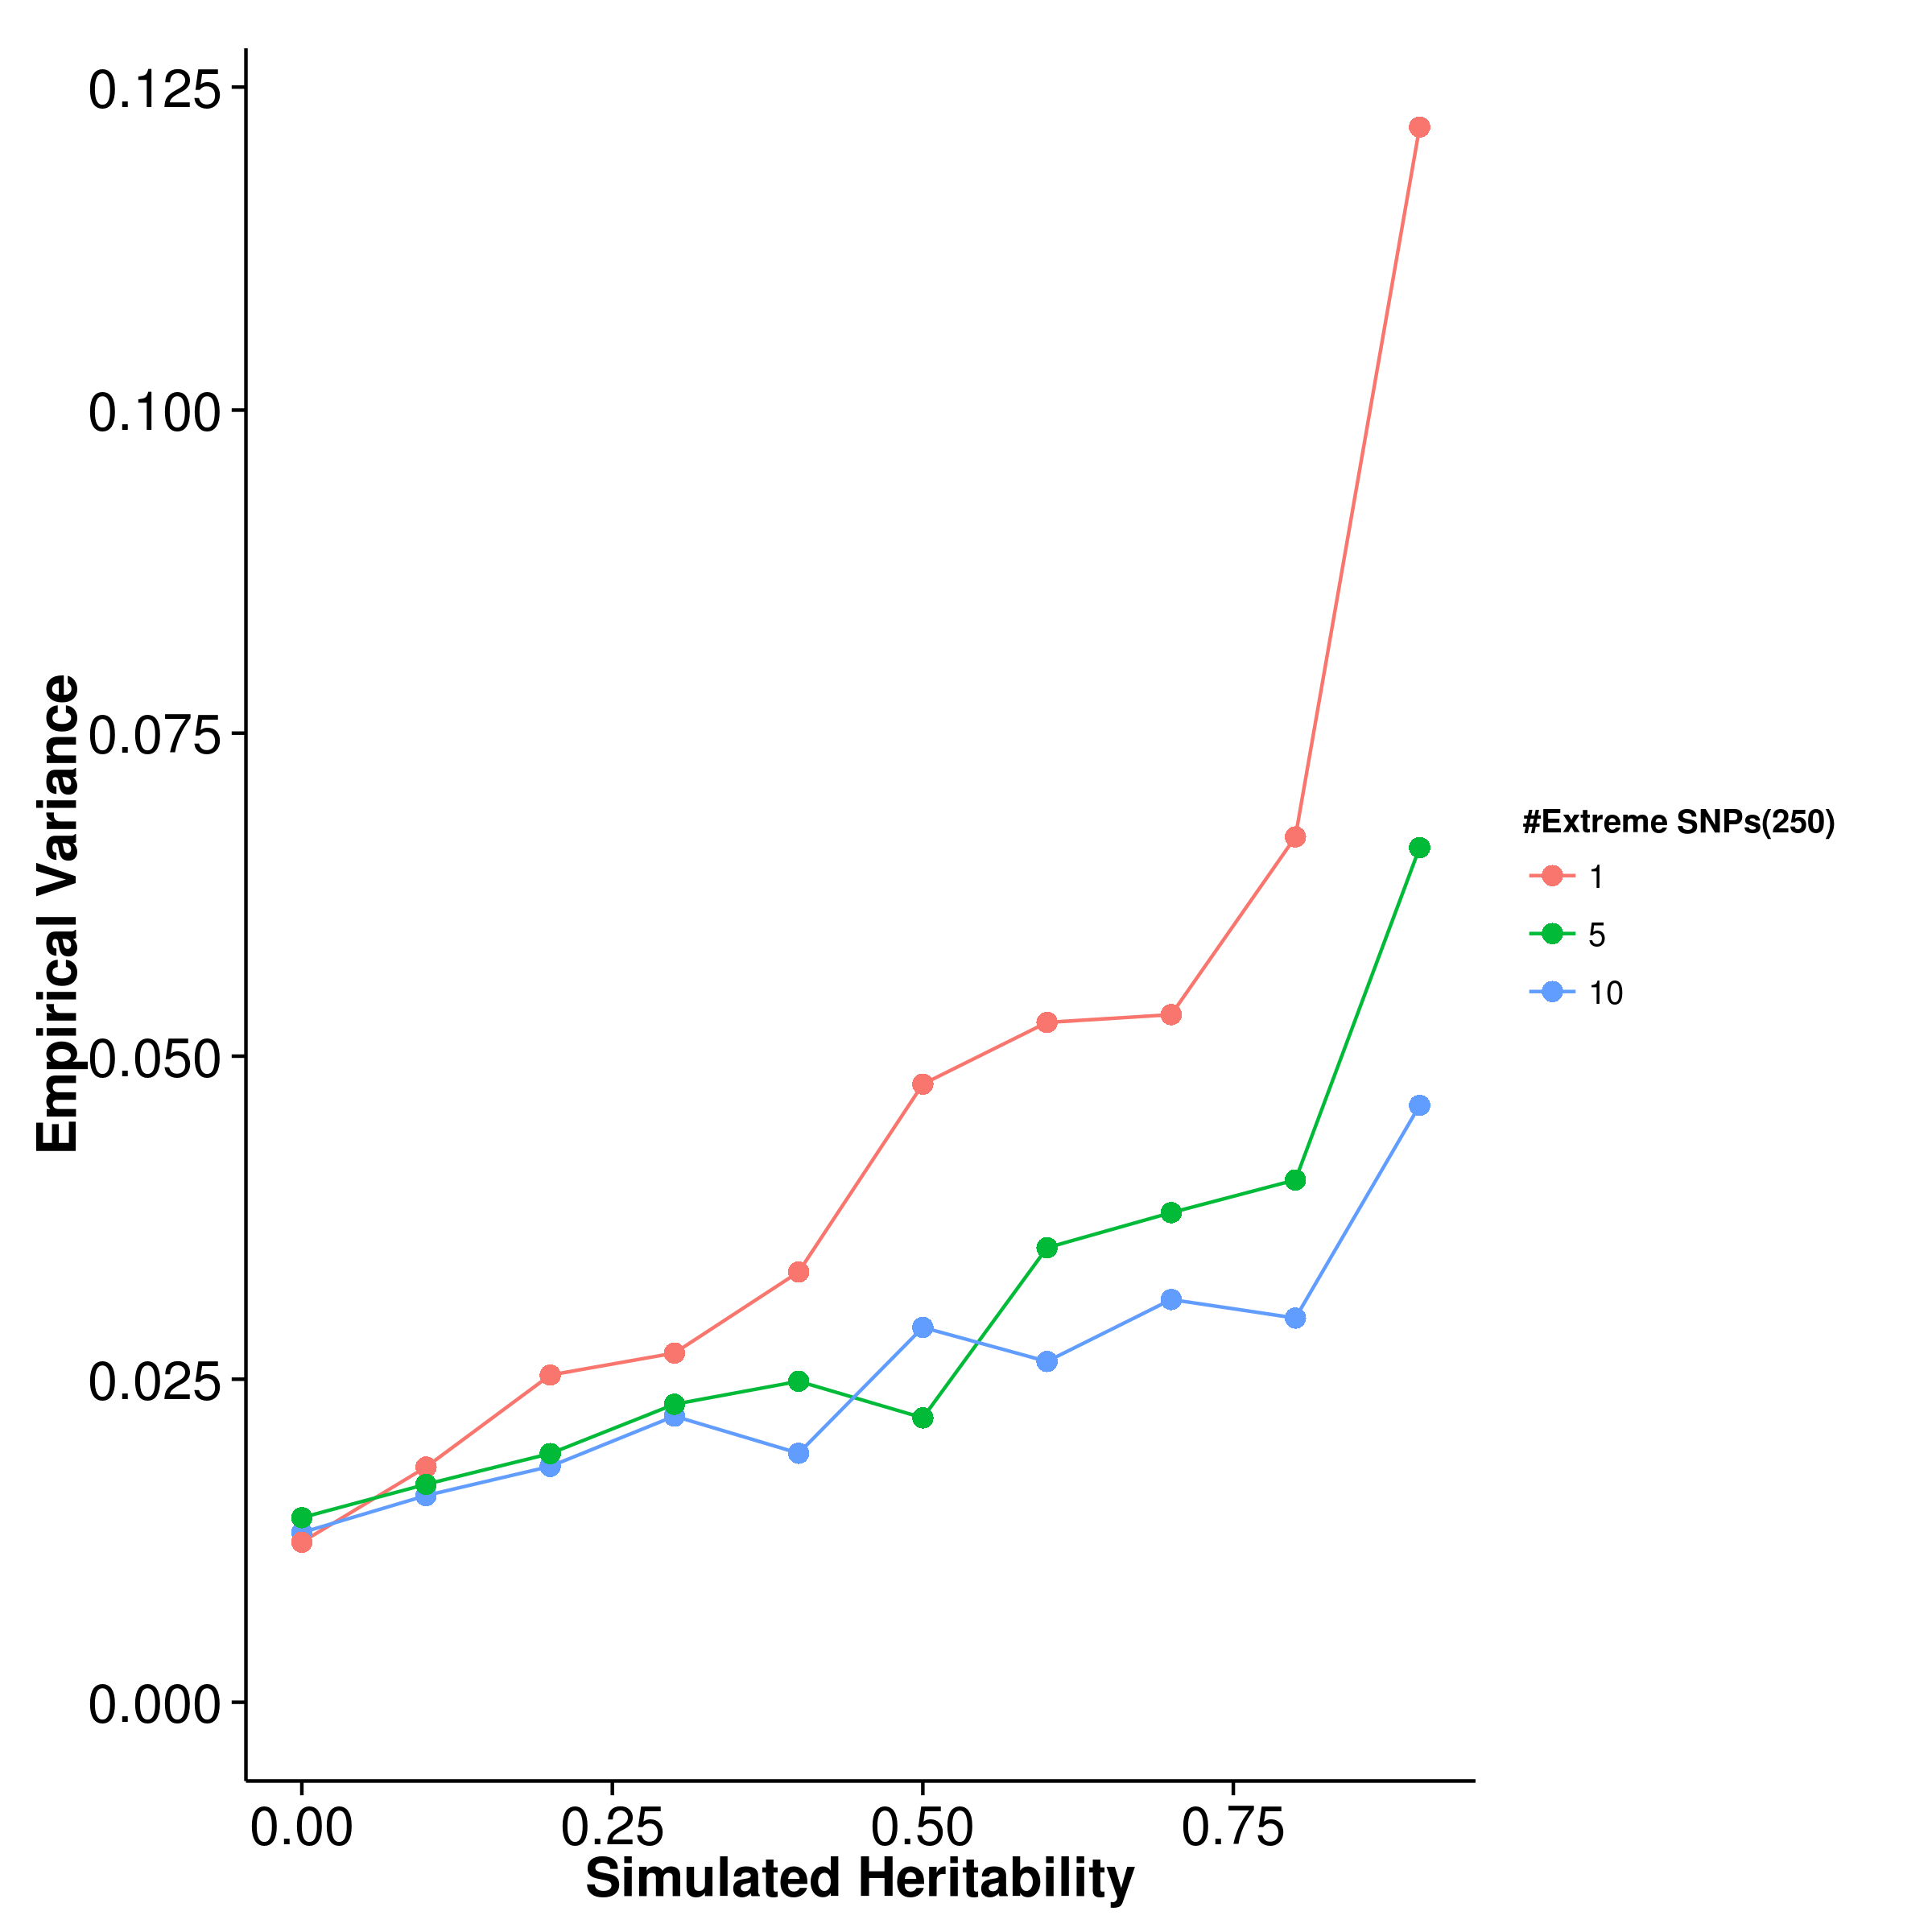
\includegraphics{figure/he_summary/extreme_250c/ldscIn_QtE_Extreme_sd.png}}
				\label{fig:ldscInQtEx250cVar}
			}
			\caption[Quantitative Trait with Extreme Effect Size Simulation Result(250 causal SNPs, Variance)]
			{Variance of results from quantitative trait simulation with extreme effect size simulation.
				250 causal \glspl{SNP} were simulated.
				Compared to the case where 100 causal \glspl{SNP} were simulated, most tools, except \gls{shrek} seems to be more sensitive to the number of \gls{SNP}(s) explaining large portion of effect, where a smaller number can lead to a higher variance.
			} 
			\label{fig:QtEx250cVar}
		\end{figure}
		
		\begin{figure}
			\centering
			\subfloat[SHREK]{
				\scalebox{.4}{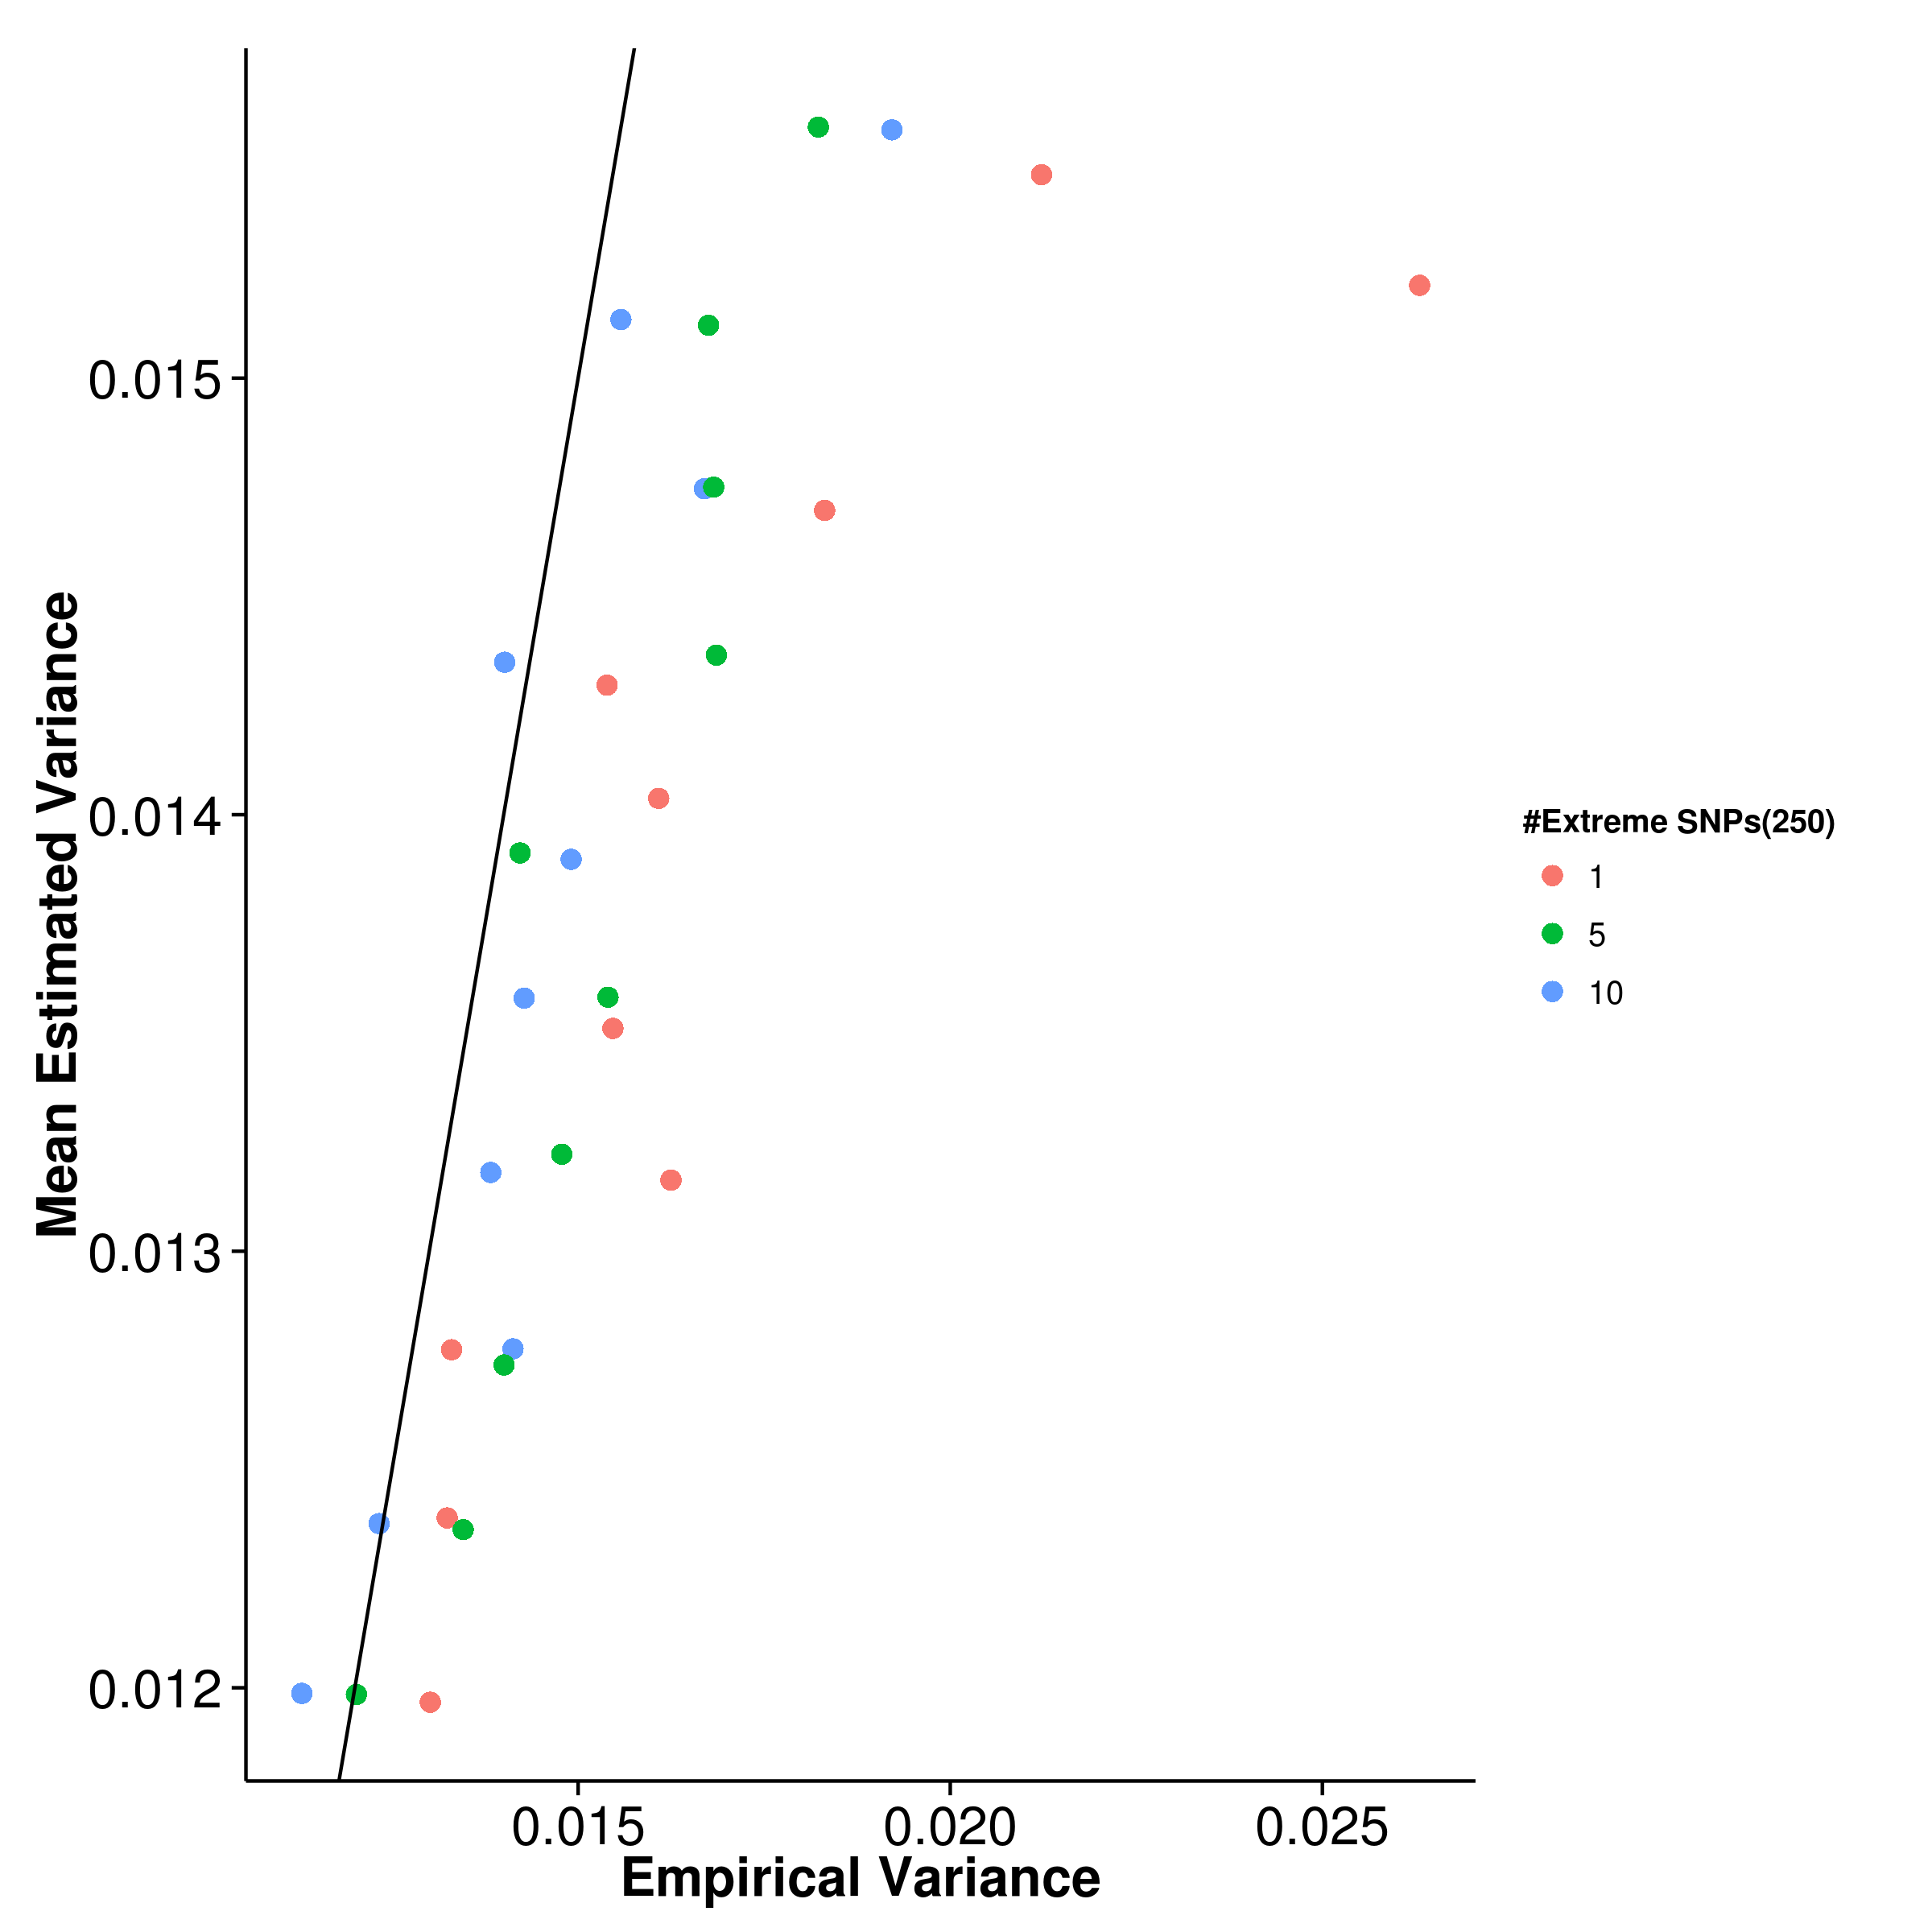
\includegraphics{figure/he_summary/extreme_250c/shrek_QtE_Extreme_sdCom.png}}
				\label{fig:shrekQtEx250cVarCom}
			}
			\subfloat[GCTA]{
				\scalebox{.4}{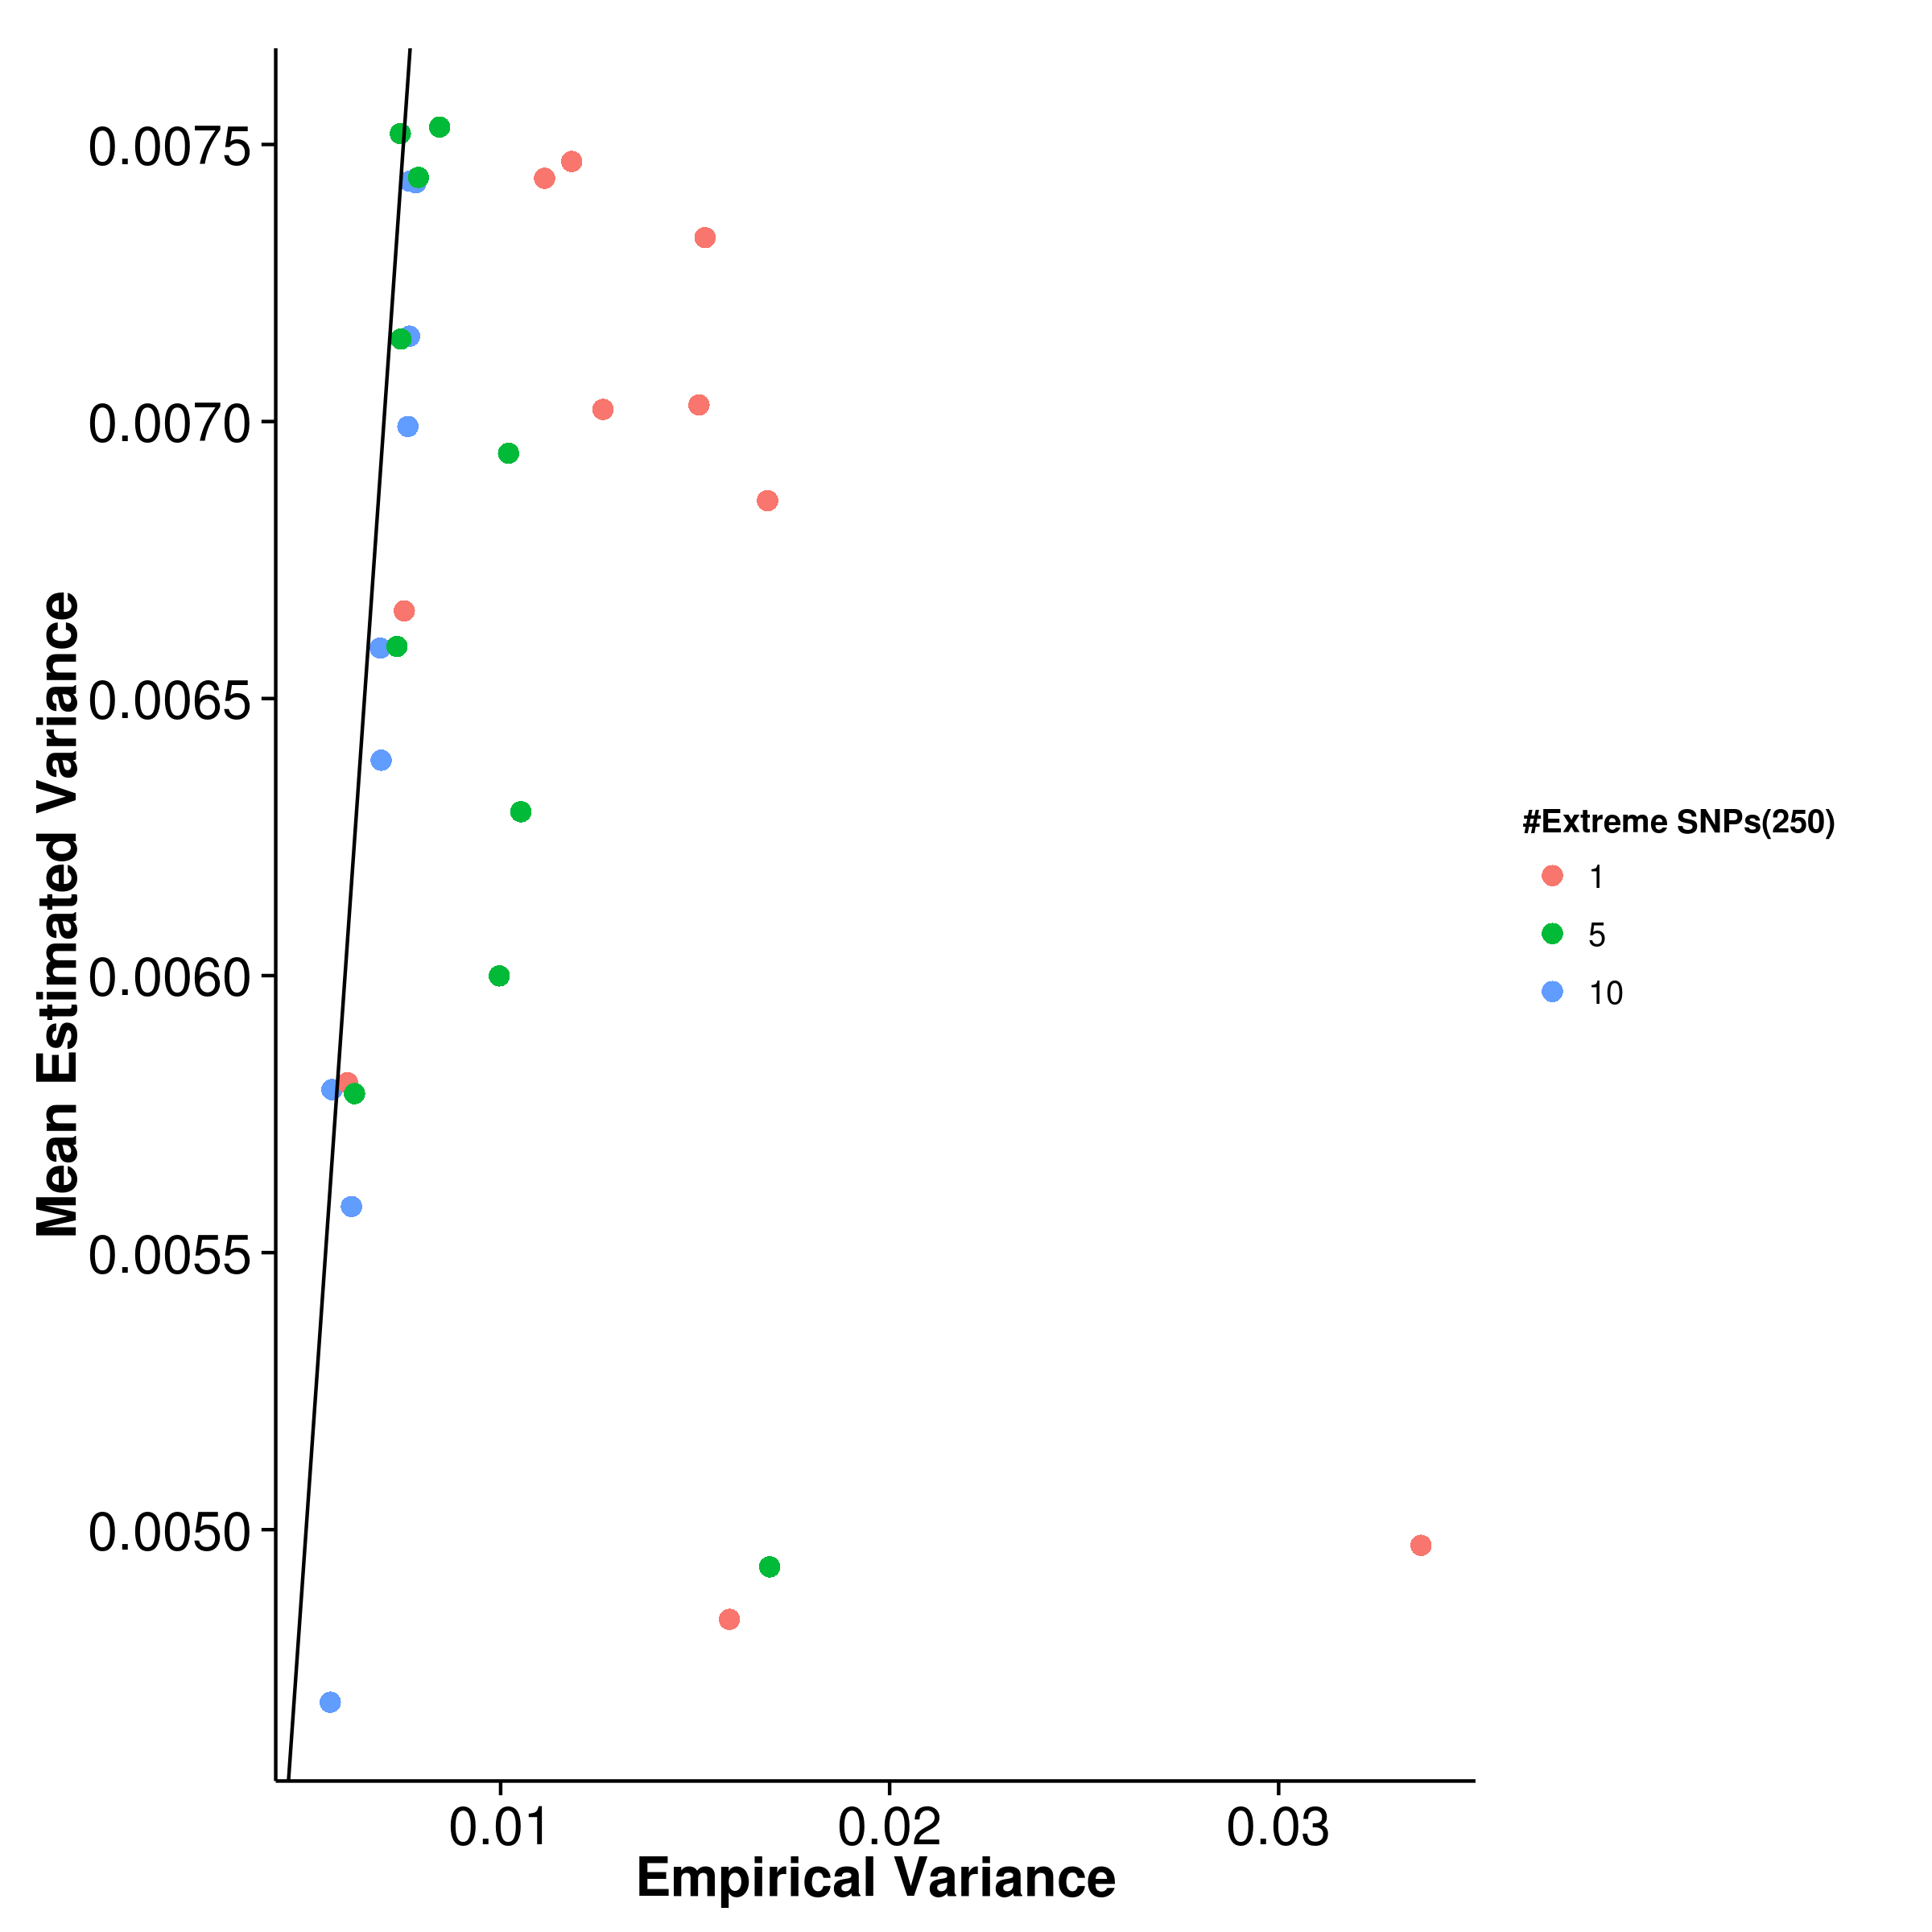
\includegraphics{figure/he_summary/extreme_250c/gcta_QtE_Extreme_sdCom.png}}
				\label{fig:gctaQtEx250cVarCom}
			}\\
			\subfloat[LDSC with fix intercept]{
				\scalebox{.4}{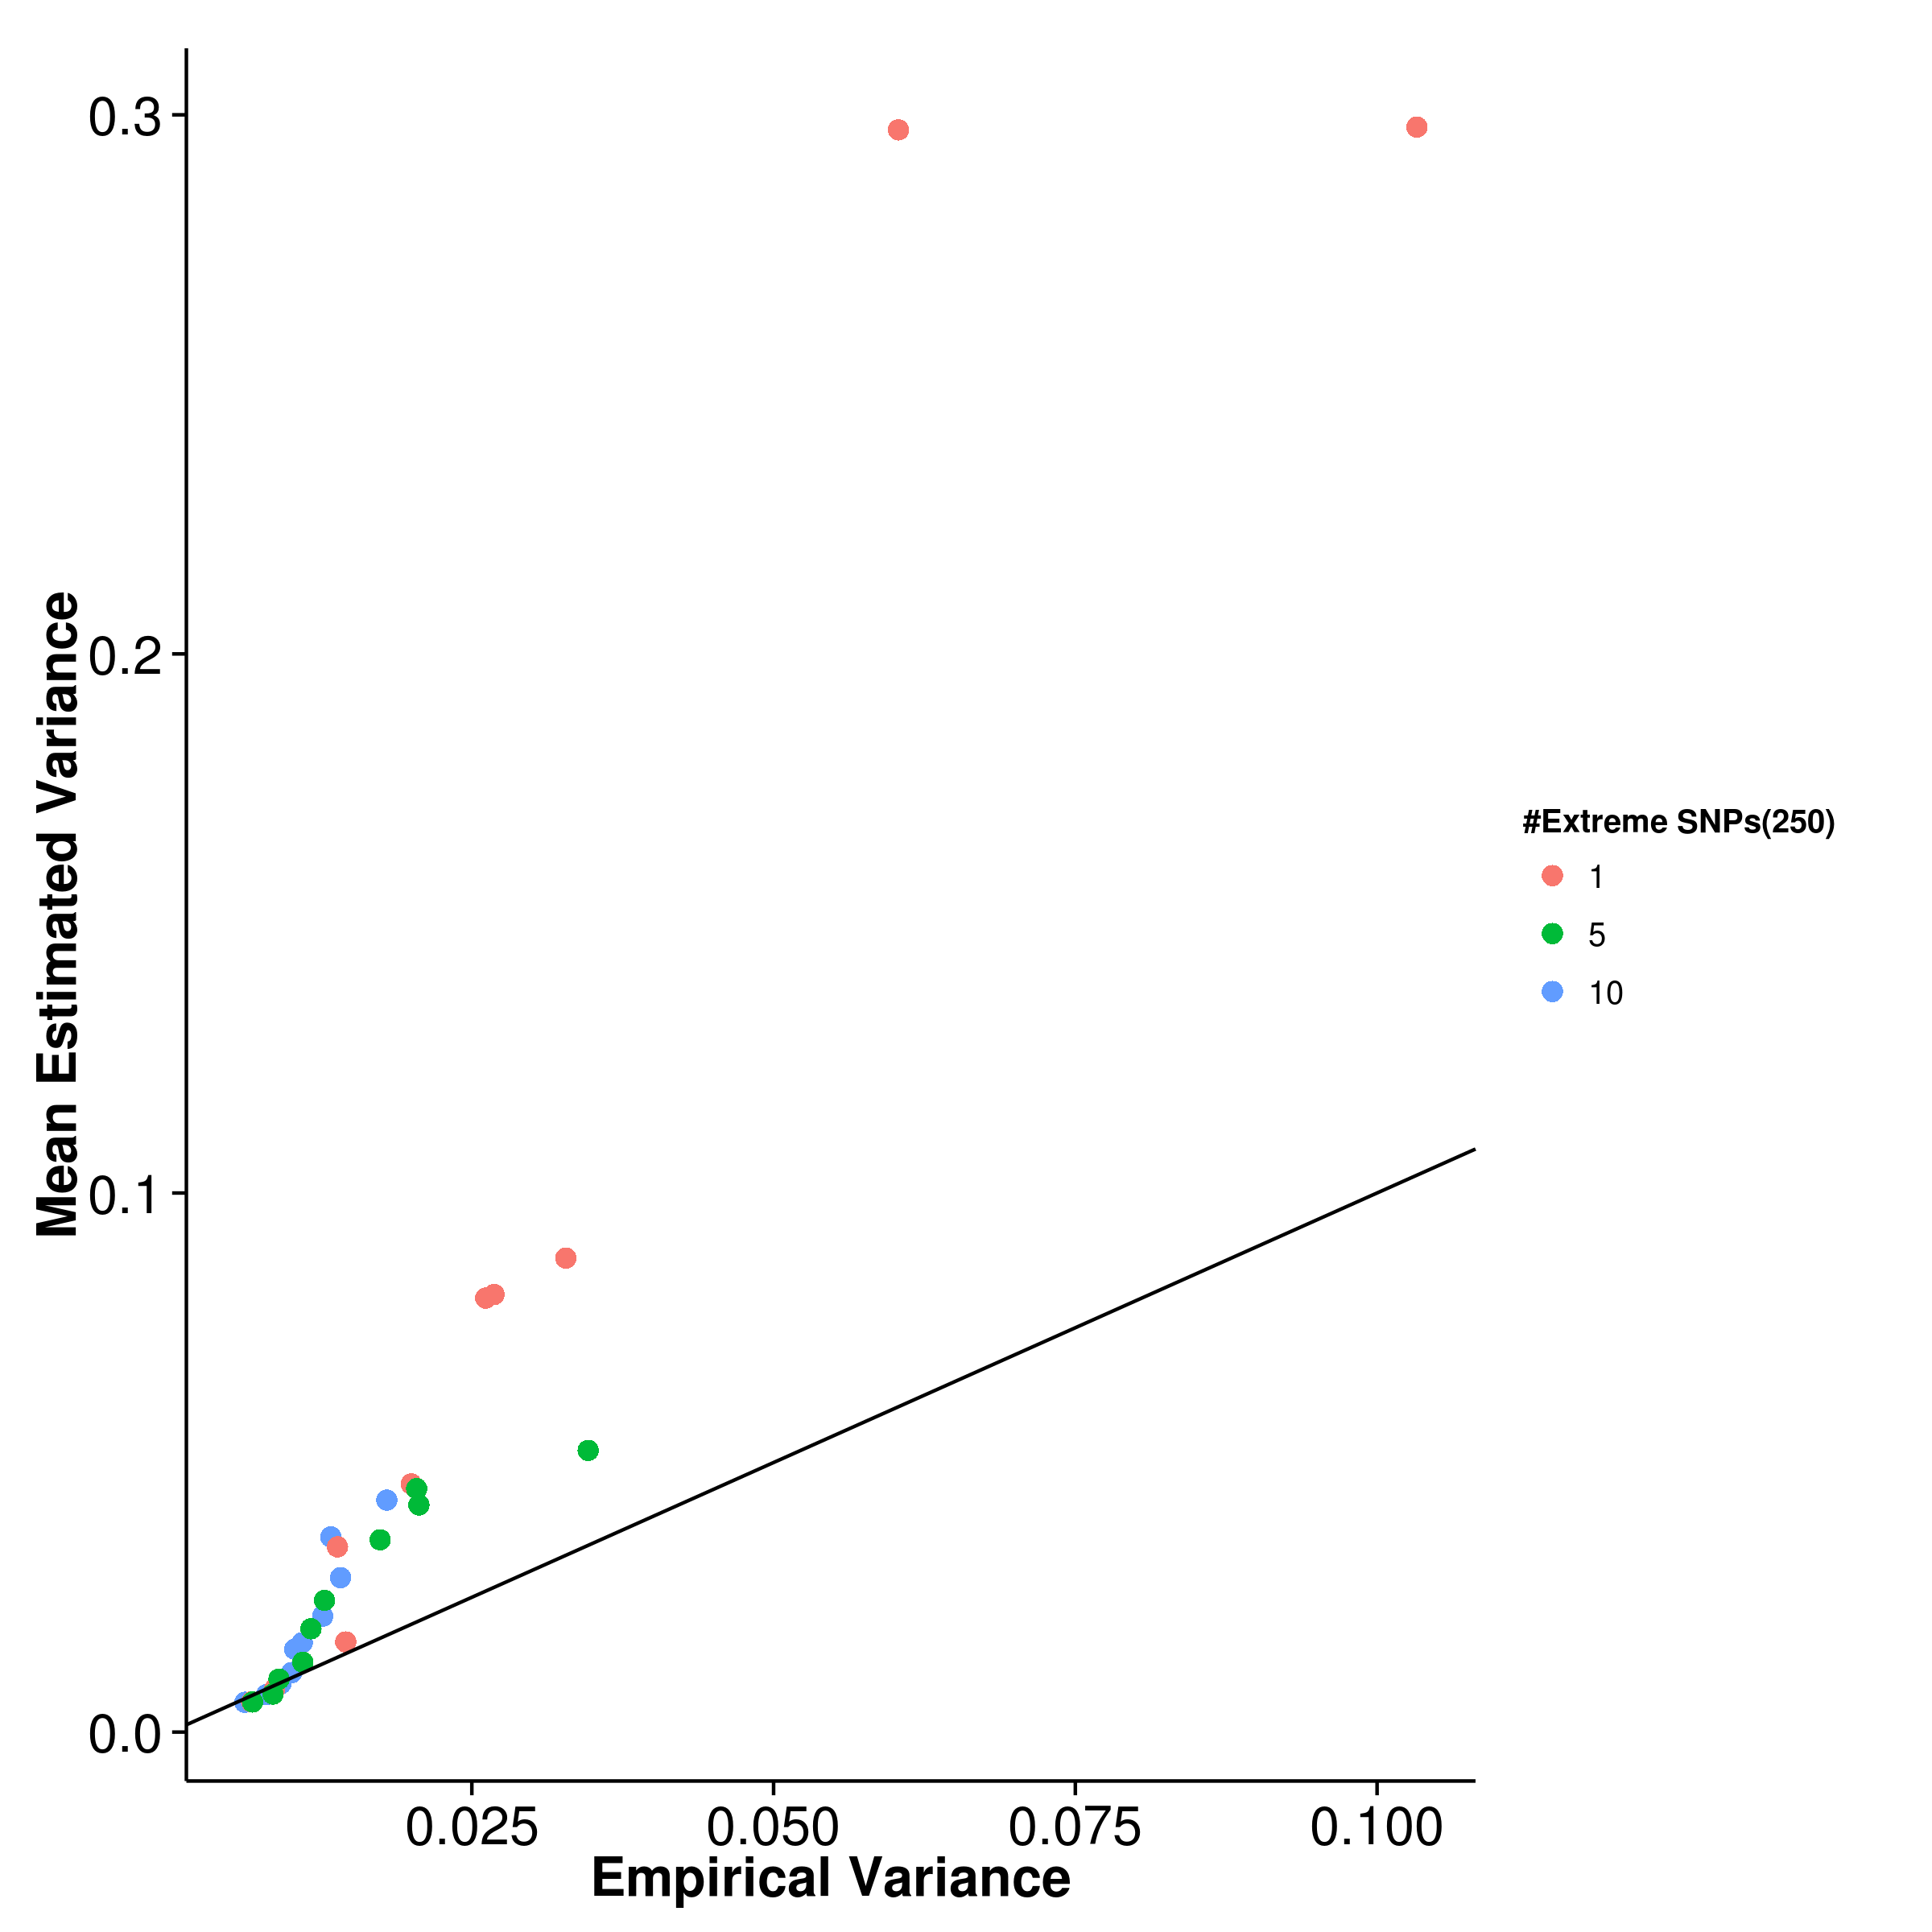
\includegraphics{figure/he_summary/extreme_250c/ldsc_QtE_Extreme_sdCom.png}}
				\label{fig:ldscQtEx250cVarCom}
			}
			\subfloat[LDSC with intercept estimation]{
				
				\scalebox{.4}{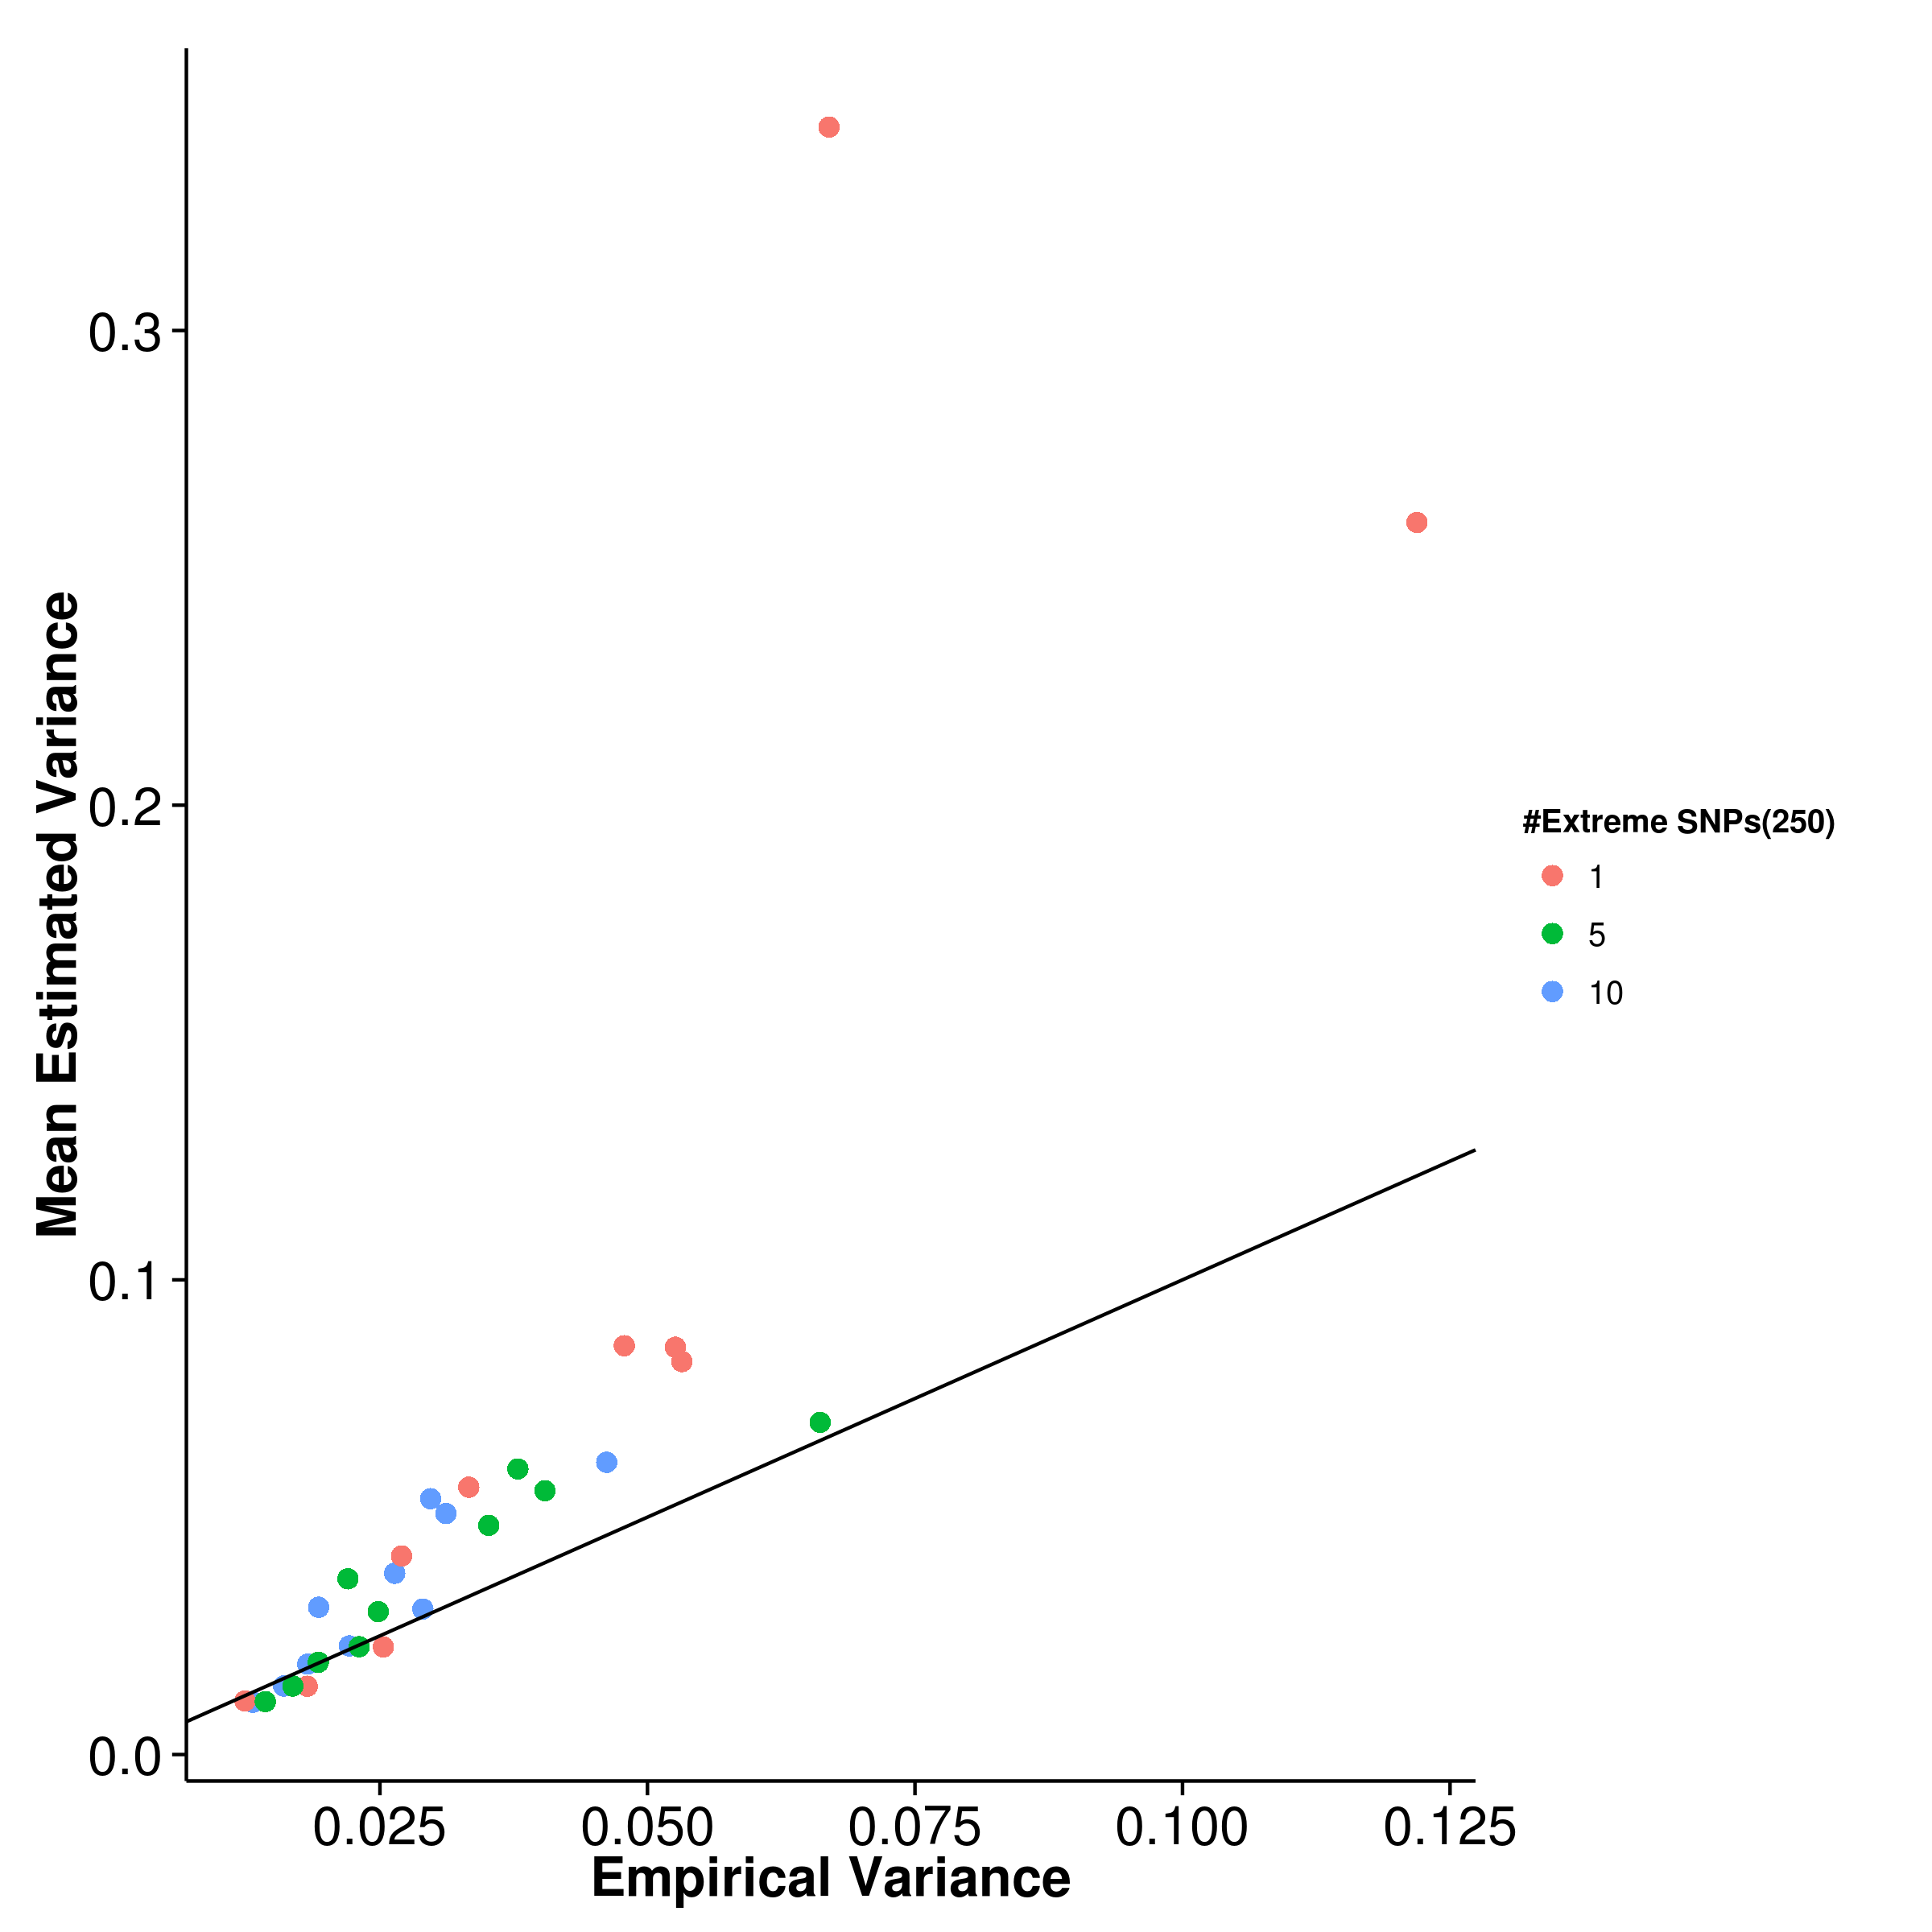
\includegraphics{figure/he_summary/extreme_250c/ldscIn_QtE_Extreme_sdCom.png}}
				\label{fig:ldscInQtEx250cVarCom}
			}
			\caption[Quantitative Trait with Extreme Effect Size Simulation Result(250 causal SNPs, Estimated Variance)]
			{Estimated variance of results from quantitative trait simulation with extreme effect size simulation when compared to the empirical variance.
				250 causal \glspl{SNP} were simulated.
				The result of simulation were the same as the previous extreme effect simulation with 100 causal \glspl{SNP}.
			} 
			\label{fig:QtEx250cVarCom}
		\end{figure}